
% Default to the notebook output style

    


% Inherit from the specified cell style.




    
\documentclass[11pt]{article}

    
    
    \usepackage[T1]{fontenc}
    % Nicer default font (+ math font) than Computer Modern for most use cases
    \usepackage{mathpazo}

    % Basic figure setup, for now with no caption control since it's done
    % automatically by Pandoc (which extracts ![](path) syntax from Markdown).
    \usepackage{graphicx}
    % We will generate all images so they have a width \maxwidth. This means
    % that they will get their normal width if they fit onto the page, but
    % are scaled down if they would overflow the margins.
    \makeatletter
    \def\maxwidth{\ifdim\Gin@nat@width>\linewidth\linewidth
    \else\Gin@nat@width\fi}
    \makeatother
    \let\Oldincludegraphics\includegraphics
    % Set max figure width to be 80% of text width, for now hardcoded.
    \renewcommand{\includegraphics}[1]{\Oldincludegraphics[width=.8\maxwidth]{#1}}
    % Ensure that by default, figures have no caption (until we provide a
    % proper Figure object with a Caption API and a way to capture that
    % in the conversion process - todo).
    \usepackage{caption}
    \DeclareCaptionLabelFormat{nolabel}{}
    \captionsetup{labelformat=nolabel}

    \usepackage{adjustbox} % Used to constrain images to a maximum size 
    \usepackage{xcolor} % Allow colors to be defined
    \usepackage{enumerate} % Needed for markdown enumerations to work
    \usepackage{geometry} % Used to adjust the document margins
    \usepackage{amsmath} % Equations
    \usepackage{amssymb} % Equations
    \usepackage{textcomp} % defines textquotesingle
    % Hack from http://tex.stackexchange.com/a/47451/13684:
    \AtBeginDocument{%
        \def\PYZsq{\textquotesingle}% Upright quotes in Pygmentized code
    }
    \usepackage{upquote} % Upright quotes for verbatim code
    \usepackage{eurosym} % defines \euro
    \usepackage[mathletters]{ucs} % Extended unicode (utf-8) support
    \usepackage[utf8x]{inputenc} % Allow utf-8 characters in the tex document
    \usepackage{fancyvrb} % verbatim replacement that allows latex
    \usepackage{grffile} % extends the file name processing of package graphics 
                         % to support a larger range 
    % The hyperref package gives us a pdf with properly built
    % internal navigation ('pdf bookmarks' for the table of contents,
    % internal cross-reference links, web links for URLs, etc.)
    \usepackage{hyperref}
    \usepackage{longtable} % longtable support required by pandoc >1.10
    \usepackage{booktabs}  % table support for pandoc > 1.12.2
    \usepackage[inline]{enumitem} % IRkernel/repr support (it uses the enumerate* environment)
    \usepackage[normalem]{ulem} % ulem is needed to support strikethroughs (\sout)
                                % normalem makes italics be italics, not underlines
    

    
    
    % Colors for the hyperref package
    \definecolor{urlcolor}{rgb}{0,.145,.698}
    \definecolor{linkcolor}{rgb}{.71,0.21,0.01}
    \definecolor{citecolor}{rgb}{.12,.54,.11}

    % ANSI colors
    \definecolor{ansi-black}{HTML}{3E424D}
    \definecolor{ansi-black-intense}{HTML}{282C36}
    \definecolor{ansi-red}{HTML}{E75C58}
    \definecolor{ansi-red-intense}{HTML}{B22B31}
    \definecolor{ansi-green}{HTML}{00A250}
    \definecolor{ansi-green-intense}{HTML}{007427}
    \definecolor{ansi-yellow}{HTML}{DDB62B}
    \definecolor{ansi-yellow-intense}{HTML}{B27D12}
    \definecolor{ansi-blue}{HTML}{208FFB}
    \definecolor{ansi-blue-intense}{HTML}{0065CA}
    \definecolor{ansi-magenta}{HTML}{D160C4}
    \definecolor{ansi-magenta-intense}{HTML}{A03196}
    \definecolor{ansi-cyan}{HTML}{60C6C8}
    \definecolor{ansi-cyan-intense}{HTML}{258F8F}
    \definecolor{ansi-white}{HTML}{C5C1B4}
    \definecolor{ansi-white-intense}{HTML}{A1A6B2}

    % commands and environments needed by pandoc snippets
    % extracted from the output of `pandoc -s`
    \providecommand{\tightlist}{%
      \setlength{\itemsep}{0pt}\setlength{\parskip}{0pt}}
    \DefineVerbatimEnvironment{Highlighting}{Verbatim}{commandchars=\\\{\}}
    % Add ',fontsize=\small' for more characters per line
    \newenvironment{Shaded}{}{}
    \newcommand{\KeywordTok}[1]{\textcolor[rgb]{0.00,0.44,0.13}{\textbf{{#1}}}}
    \newcommand{\DataTypeTok}[1]{\textcolor[rgb]{0.56,0.13,0.00}{{#1}}}
    \newcommand{\DecValTok}[1]{\textcolor[rgb]{0.25,0.63,0.44}{{#1}}}
    \newcommand{\BaseNTok}[1]{\textcolor[rgb]{0.25,0.63,0.44}{{#1}}}
    \newcommand{\FloatTok}[1]{\textcolor[rgb]{0.25,0.63,0.44}{{#1}}}
    \newcommand{\CharTok}[1]{\textcolor[rgb]{0.25,0.44,0.63}{{#1}}}
    \newcommand{\StringTok}[1]{\textcolor[rgb]{0.25,0.44,0.63}{{#1}}}
    \newcommand{\CommentTok}[1]{\textcolor[rgb]{0.38,0.63,0.69}{\textit{{#1}}}}
    \newcommand{\OtherTok}[1]{\textcolor[rgb]{0.00,0.44,0.13}{{#1}}}
    \newcommand{\AlertTok}[1]{\textcolor[rgb]{1.00,0.00,0.00}{\textbf{{#1}}}}
    \newcommand{\FunctionTok}[1]{\textcolor[rgb]{0.02,0.16,0.49}{{#1}}}
    \newcommand{\RegionMarkerTok}[1]{{#1}}
    \newcommand{\ErrorTok}[1]{\textcolor[rgb]{1.00,0.00,0.00}{\textbf{{#1}}}}
    \newcommand{\NormalTok}[1]{{#1}}
    
    % Additional commands for more recent versions of Pandoc
    \newcommand{\ConstantTok}[1]{\textcolor[rgb]{0.53,0.00,0.00}{{#1}}}
    \newcommand{\SpecialCharTok}[1]{\textcolor[rgb]{0.25,0.44,0.63}{{#1}}}
    \newcommand{\VerbatimStringTok}[1]{\textcolor[rgb]{0.25,0.44,0.63}{{#1}}}
    \newcommand{\SpecialStringTok}[1]{\textcolor[rgb]{0.73,0.40,0.53}{{#1}}}
    \newcommand{\ImportTok}[1]{{#1}}
    \newcommand{\DocumentationTok}[1]{\textcolor[rgb]{0.73,0.13,0.13}{\textit{{#1}}}}
    \newcommand{\AnnotationTok}[1]{\textcolor[rgb]{0.38,0.63,0.69}{\textbf{\textit{{#1}}}}}
    \newcommand{\CommentVarTok}[1]{\textcolor[rgb]{0.38,0.63,0.69}{\textbf{\textit{{#1}}}}}
    \newcommand{\VariableTok}[1]{\textcolor[rgb]{0.10,0.09,0.49}{{#1}}}
    \newcommand{\ControlFlowTok}[1]{\textcolor[rgb]{0.00,0.44,0.13}{\textbf{{#1}}}}
    \newcommand{\OperatorTok}[1]{\textcolor[rgb]{0.40,0.40,0.40}{{#1}}}
    \newcommand{\BuiltInTok}[1]{{#1}}
    \newcommand{\ExtensionTok}[1]{{#1}}
    \newcommand{\PreprocessorTok}[1]{\textcolor[rgb]{0.74,0.48,0.00}{{#1}}}
    \newcommand{\AttributeTok}[1]{\textcolor[rgb]{0.49,0.56,0.16}{{#1}}}
    \newcommand{\InformationTok}[1]{\textcolor[rgb]{0.38,0.63,0.69}{\textbf{\textit{{#1}}}}}
    \newcommand{\WarningTok}[1]{\textcolor[rgb]{0.38,0.63,0.69}{\textbf{\textit{{#1}}}}}
    
    
    % Define a nice break command that doesn't care if a line doesn't already
    % exist.
    \def\br{\hspace*{\fill} \\* }
    % Math Jax compatability definitions
    \def\gt{>}
    \def\lt{<}
    % Document parameters
    \title{v2}
    
    
    

    % Pygments definitions
    
\makeatletter
\def\PY@reset{\let\PY@it=\relax \let\PY@bf=\relax%
    \let\PY@ul=\relax \let\PY@tc=\relax%
    \let\PY@bc=\relax \let\PY@ff=\relax}
\def\PY@tok#1{\csname PY@tok@#1\endcsname}
\def\PY@toks#1+{\ifx\relax#1\empty\else%
    \PY@tok{#1}\expandafter\PY@toks\fi}
\def\PY@do#1{\PY@bc{\PY@tc{\PY@ul{%
    \PY@it{\PY@bf{\PY@ff{#1}}}}}}}
\def\PY#1#2{\PY@reset\PY@toks#1+\relax+\PY@do{#2}}

\expandafter\def\csname PY@tok@w\endcsname{\def\PY@tc##1{\textcolor[rgb]{0.73,0.73,0.73}{##1}}}
\expandafter\def\csname PY@tok@c\endcsname{\let\PY@it=\textit\def\PY@tc##1{\textcolor[rgb]{0.25,0.50,0.50}{##1}}}
\expandafter\def\csname PY@tok@cp\endcsname{\def\PY@tc##1{\textcolor[rgb]{0.74,0.48,0.00}{##1}}}
\expandafter\def\csname PY@tok@k\endcsname{\let\PY@bf=\textbf\def\PY@tc##1{\textcolor[rgb]{0.00,0.50,0.00}{##1}}}
\expandafter\def\csname PY@tok@kp\endcsname{\def\PY@tc##1{\textcolor[rgb]{0.00,0.50,0.00}{##1}}}
\expandafter\def\csname PY@tok@kt\endcsname{\def\PY@tc##1{\textcolor[rgb]{0.69,0.00,0.25}{##1}}}
\expandafter\def\csname PY@tok@o\endcsname{\def\PY@tc##1{\textcolor[rgb]{0.40,0.40,0.40}{##1}}}
\expandafter\def\csname PY@tok@ow\endcsname{\let\PY@bf=\textbf\def\PY@tc##1{\textcolor[rgb]{0.67,0.13,1.00}{##1}}}
\expandafter\def\csname PY@tok@nb\endcsname{\def\PY@tc##1{\textcolor[rgb]{0.00,0.50,0.00}{##1}}}
\expandafter\def\csname PY@tok@nf\endcsname{\def\PY@tc##1{\textcolor[rgb]{0.00,0.00,1.00}{##1}}}
\expandafter\def\csname PY@tok@nc\endcsname{\let\PY@bf=\textbf\def\PY@tc##1{\textcolor[rgb]{0.00,0.00,1.00}{##1}}}
\expandafter\def\csname PY@tok@nn\endcsname{\let\PY@bf=\textbf\def\PY@tc##1{\textcolor[rgb]{0.00,0.00,1.00}{##1}}}
\expandafter\def\csname PY@tok@ne\endcsname{\let\PY@bf=\textbf\def\PY@tc##1{\textcolor[rgb]{0.82,0.25,0.23}{##1}}}
\expandafter\def\csname PY@tok@nv\endcsname{\def\PY@tc##1{\textcolor[rgb]{0.10,0.09,0.49}{##1}}}
\expandafter\def\csname PY@tok@no\endcsname{\def\PY@tc##1{\textcolor[rgb]{0.53,0.00,0.00}{##1}}}
\expandafter\def\csname PY@tok@nl\endcsname{\def\PY@tc##1{\textcolor[rgb]{0.63,0.63,0.00}{##1}}}
\expandafter\def\csname PY@tok@ni\endcsname{\let\PY@bf=\textbf\def\PY@tc##1{\textcolor[rgb]{0.60,0.60,0.60}{##1}}}
\expandafter\def\csname PY@tok@na\endcsname{\def\PY@tc##1{\textcolor[rgb]{0.49,0.56,0.16}{##1}}}
\expandafter\def\csname PY@tok@nt\endcsname{\let\PY@bf=\textbf\def\PY@tc##1{\textcolor[rgb]{0.00,0.50,0.00}{##1}}}
\expandafter\def\csname PY@tok@nd\endcsname{\def\PY@tc##1{\textcolor[rgb]{0.67,0.13,1.00}{##1}}}
\expandafter\def\csname PY@tok@s\endcsname{\def\PY@tc##1{\textcolor[rgb]{0.73,0.13,0.13}{##1}}}
\expandafter\def\csname PY@tok@sd\endcsname{\let\PY@it=\textit\def\PY@tc##1{\textcolor[rgb]{0.73,0.13,0.13}{##1}}}
\expandafter\def\csname PY@tok@si\endcsname{\let\PY@bf=\textbf\def\PY@tc##1{\textcolor[rgb]{0.73,0.40,0.53}{##1}}}
\expandafter\def\csname PY@tok@se\endcsname{\let\PY@bf=\textbf\def\PY@tc##1{\textcolor[rgb]{0.73,0.40,0.13}{##1}}}
\expandafter\def\csname PY@tok@sr\endcsname{\def\PY@tc##1{\textcolor[rgb]{0.73,0.40,0.53}{##1}}}
\expandafter\def\csname PY@tok@ss\endcsname{\def\PY@tc##1{\textcolor[rgb]{0.10,0.09,0.49}{##1}}}
\expandafter\def\csname PY@tok@sx\endcsname{\def\PY@tc##1{\textcolor[rgb]{0.00,0.50,0.00}{##1}}}
\expandafter\def\csname PY@tok@m\endcsname{\def\PY@tc##1{\textcolor[rgb]{0.40,0.40,0.40}{##1}}}
\expandafter\def\csname PY@tok@gh\endcsname{\let\PY@bf=\textbf\def\PY@tc##1{\textcolor[rgb]{0.00,0.00,0.50}{##1}}}
\expandafter\def\csname PY@tok@gu\endcsname{\let\PY@bf=\textbf\def\PY@tc##1{\textcolor[rgb]{0.50,0.00,0.50}{##1}}}
\expandafter\def\csname PY@tok@gd\endcsname{\def\PY@tc##1{\textcolor[rgb]{0.63,0.00,0.00}{##1}}}
\expandafter\def\csname PY@tok@gi\endcsname{\def\PY@tc##1{\textcolor[rgb]{0.00,0.63,0.00}{##1}}}
\expandafter\def\csname PY@tok@gr\endcsname{\def\PY@tc##1{\textcolor[rgb]{1.00,0.00,0.00}{##1}}}
\expandafter\def\csname PY@tok@ge\endcsname{\let\PY@it=\textit}
\expandafter\def\csname PY@tok@gs\endcsname{\let\PY@bf=\textbf}
\expandafter\def\csname PY@tok@gp\endcsname{\let\PY@bf=\textbf\def\PY@tc##1{\textcolor[rgb]{0.00,0.00,0.50}{##1}}}
\expandafter\def\csname PY@tok@go\endcsname{\def\PY@tc##1{\textcolor[rgb]{0.53,0.53,0.53}{##1}}}
\expandafter\def\csname PY@tok@gt\endcsname{\def\PY@tc##1{\textcolor[rgb]{0.00,0.27,0.87}{##1}}}
\expandafter\def\csname PY@tok@err\endcsname{\def\PY@bc##1{\setlength{\fboxsep}{0pt}\fcolorbox[rgb]{1.00,0.00,0.00}{1,1,1}{\strut ##1}}}
\expandafter\def\csname PY@tok@kc\endcsname{\let\PY@bf=\textbf\def\PY@tc##1{\textcolor[rgb]{0.00,0.50,0.00}{##1}}}
\expandafter\def\csname PY@tok@kd\endcsname{\let\PY@bf=\textbf\def\PY@tc##1{\textcolor[rgb]{0.00,0.50,0.00}{##1}}}
\expandafter\def\csname PY@tok@kn\endcsname{\let\PY@bf=\textbf\def\PY@tc##1{\textcolor[rgb]{0.00,0.50,0.00}{##1}}}
\expandafter\def\csname PY@tok@kr\endcsname{\let\PY@bf=\textbf\def\PY@tc##1{\textcolor[rgb]{0.00,0.50,0.00}{##1}}}
\expandafter\def\csname PY@tok@bp\endcsname{\def\PY@tc##1{\textcolor[rgb]{0.00,0.50,0.00}{##1}}}
\expandafter\def\csname PY@tok@fm\endcsname{\def\PY@tc##1{\textcolor[rgb]{0.00,0.00,1.00}{##1}}}
\expandafter\def\csname PY@tok@vc\endcsname{\def\PY@tc##1{\textcolor[rgb]{0.10,0.09,0.49}{##1}}}
\expandafter\def\csname PY@tok@vg\endcsname{\def\PY@tc##1{\textcolor[rgb]{0.10,0.09,0.49}{##1}}}
\expandafter\def\csname PY@tok@vi\endcsname{\def\PY@tc##1{\textcolor[rgb]{0.10,0.09,0.49}{##1}}}
\expandafter\def\csname PY@tok@vm\endcsname{\def\PY@tc##1{\textcolor[rgb]{0.10,0.09,0.49}{##1}}}
\expandafter\def\csname PY@tok@sa\endcsname{\def\PY@tc##1{\textcolor[rgb]{0.73,0.13,0.13}{##1}}}
\expandafter\def\csname PY@tok@sb\endcsname{\def\PY@tc##1{\textcolor[rgb]{0.73,0.13,0.13}{##1}}}
\expandafter\def\csname PY@tok@sc\endcsname{\def\PY@tc##1{\textcolor[rgb]{0.73,0.13,0.13}{##1}}}
\expandafter\def\csname PY@tok@dl\endcsname{\def\PY@tc##1{\textcolor[rgb]{0.73,0.13,0.13}{##1}}}
\expandafter\def\csname PY@tok@s2\endcsname{\def\PY@tc##1{\textcolor[rgb]{0.73,0.13,0.13}{##1}}}
\expandafter\def\csname PY@tok@sh\endcsname{\def\PY@tc##1{\textcolor[rgb]{0.73,0.13,0.13}{##1}}}
\expandafter\def\csname PY@tok@s1\endcsname{\def\PY@tc##1{\textcolor[rgb]{0.73,0.13,0.13}{##1}}}
\expandafter\def\csname PY@tok@mb\endcsname{\def\PY@tc##1{\textcolor[rgb]{0.40,0.40,0.40}{##1}}}
\expandafter\def\csname PY@tok@mf\endcsname{\def\PY@tc##1{\textcolor[rgb]{0.40,0.40,0.40}{##1}}}
\expandafter\def\csname PY@tok@mh\endcsname{\def\PY@tc##1{\textcolor[rgb]{0.40,0.40,0.40}{##1}}}
\expandafter\def\csname PY@tok@mi\endcsname{\def\PY@tc##1{\textcolor[rgb]{0.40,0.40,0.40}{##1}}}
\expandafter\def\csname PY@tok@il\endcsname{\def\PY@tc##1{\textcolor[rgb]{0.40,0.40,0.40}{##1}}}
\expandafter\def\csname PY@tok@mo\endcsname{\def\PY@tc##1{\textcolor[rgb]{0.40,0.40,0.40}{##1}}}
\expandafter\def\csname PY@tok@ch\endcsname{\let\PY@it=\textit\def\PY@tc##1{\textcolor[rgb]{0.25,0.50,0.50}{##1}}}
\expandafter\def\csname PY@tok@cm\endcsname{\let\PY@it=\textit\def\PY@tc##1{\textcolor[rgb]{0.25,0.50,0.50}{##1}}}
\expandafter\def\csname PY@tok@cpf\endcsname{\let\PY@it=\textit\def\PY@tc##1{\textcolor[rgb]{0.25,0.50,0.50}{##1}}}
\expandafter\def\csname PY@tok@c1\endcsname{\let\PY@it=\textit\def\PY@tc##1{\textcolor[rgb]{0.25,0.50,0.50}{##1}}}
\expandafter\def\csname PY@tok@cs\endcsname{\let\PY@it=\textit\def\PY@tc##1{\textcolor[rgb]{0.25,0.50,0.50}{##1}}}

\def\PYZbs{\char`\\}
\def\PYZus{\char`\_}
\def\PYZob{\char`\{}
\def\PYZcb{\char`\}}
\def\PYZca{\char`\^}
\def\PYZam{\char`\&}
\def\PYZlt{\char`\<}
\def\PYZgt{\char`\>}
\def\PYZsh{\char`\#}
\def\PYZpc{\char`\%}
\def\PYZdl{\char`\$}
\def\PYZhy{\char`\-}
\def\PYZsq{\char`\'}
\def\PYZdq{\char`\"}
\def\PYZti{\char`\~}
% for compatibility with earlier versions
\def\PYZat{@}
\def\PYZlb{[}
\def\PYZrb{]}
\makeatother


    % Exact colors from NB
    \definecolor{incolor}{rgb}{0.0, 0.0, 0.5}
    \definecolor{outcolor}{rgb}{0.545, 0.0, 0.0}



    
    % Prevent overflowing lines due to hard-to-break entities
    \sloppy 
    % Setup hyperref package
    \hypersetup{
      breaklinks=true,  % so long urls are correctly broken across lines
      colorlinks=true,
      urlcolor=urlcolor,
      linkcolor=linkcolor,
      citecolor=citecolor,
      }
    % Slightly bigger margins than the latex defaults
    
    \geometry{verbose,tmargin=1in,bmargin=1in,lmargin=1in,rmargin=1in}
    
    

    \begin{document}
    
    
    \maketitle
    
    

    
    

    \section{Verkefni II}\label{verkefni-ii}

\subsubsection{Motion Control in Computer-Aided
Modeling}\label{motion-control-in-computer-aided-modeling}

\subparagraph{Reality Check 5, Numerical Analysis 2nd ed.,
Sauer.}\label{reality-check-5-numerical-analysis-2nd-ed.-sauer.}

\paragraph{Erling Óskar Kristjánsson,
eok4@hi.is}\label{erling-uxf3skar-kristjuxe1nsson-eok4hi.is}

\paragraph{Davíð Freyr Björnsson,
dfb2@hi.is}\label{davuxeduxf0-freyr-bjuxf6rnsson-dfb2hi.is}

\subparagraph{Námskeið: Töluleg Greining
(Stæ405G)}\label{nuxe1mskeiuxf0-tuxf6luleg-greining-stuxe6405g}

\subparagraph{Stofnun: Háskóli
Íslands}\label{stofnun-huxe1skuxf3li-uxedslands}

\subparagraph{Umsjónamaður: Sigurður Freyr
Hafstein}\label{umsjuxf3namauxf0ur-siguruxf0ur-freyr-hafstein}

\subparagraph{Vor 2019}\label{vor-2019}

    Introduction

Computer-aided modeling and manufacturing requires precise control of
spatial position along a prescribed motion path. We will illustrate the
use of Adaptive Quadrature to solve a fundamental piece of the problem:
equipartition, or the division of an arbitrary path into equal-length
subpaths.

In numerical machining problems, it is preferable to maintain constant
speed along the path. During each second, progress should be made along
an equal length of the machine-- material interface. In other motion
planning applications, including computer animation, more complicated
progress curves may be required: A hand reaching for a doorknob might
begin and end with low velocity and have higher velocity in between.
Robotics and virtual reality applications require the construction of
parametrized curves and surfaces to be navigated. Building a table of
small equal increments in path distance is often a necessary first step.

Assume that a parametric path P =
\(\{x(t),\ y(t) \ | \  0 \leq t \leq 1\}\) is given. Figure 5.6 shows
the example path

\[
P =
\begin{cases}
x(t) = 0.5 + 0.3t + 3.9t^2 − 4.7t^3, \\
y(t) = 1.5 + 0.3t + 0.9t^2 − 2.7t^3
\end{cases}
\]

Bézier curve defined by the four points \((0.5,1.5)\), \((0.6,1.6)\),
\((2,2)\), \((0,0)\). Points defined by evenly spaced parameter values
\(t = 0, 1/4, 1/2, 3/4, 1\) are shown.

\begin{figure}
\centering
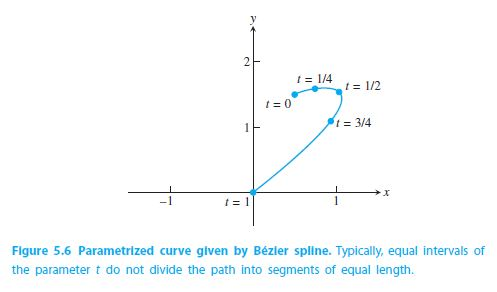
\includegraphics{img/Figure5_6.JPG}
\caption{(May need to host pictures like this online and supply a https
link) Figure 5.6}
\end{figure}

Note that even spacing in parameter does not imply even spacing in arc
length. Your goal is to apply quadrature methods to divide this path
into \(n\) equal lengths.

Recall from calculus that the arc length of the path from \(t_1\) to
\(t_2\) is

\[
\int_{t_1}^{t_2} \sqrt{x'(t)^2+y'(t)^2}dt
\]

Only rarely does the integral yield a closed-form expression, and
normally an Adaptive Quadrature technique is used to control the
parametrization of the path.

    \subsection{Preliminaries}\label{preliminaries}

Commence by defining global imports, the given parametric function and
its curve, as well as a global tolerance and the number of decimal
places that will be specified throughout the project.

    \begin{Verbatim}[commandchars=\\\{\}]
{\color{incolor}In [{\color{incolor}1}]:} \PY{l+s+sd}{\PYZdq{}\PYZdq{}\PYZdq{} Global Imports \PYZdq{}\PYZdq{}\PYZdq{}}
        \PY{c+c1}{\PYZsh{} Plots and animation}
        \PY{k+kn}{import} \PY{n+nn}{matplotlib}
        \PY{k+kn}{from} \PY{n+nn}{matplotlib}\PY{n+nn}{.}\PY{n+nn}{backends}\PY{n+nn}{.}\PY{n+nn}{backend\PYZus{}agg} \PY{k}{import} \PY{n}{FigureCanvasAgg}
        \PY{k+kn}{from} \PY{n+nn}{mpl\PYZus{}toolkits}\PY{n+nn}{.}\PY{n+nn}{mplot3d} \PY{k}{import} \PY{n}{Axes3D}
        \PY{k+kn}{from} \PY{n+nn}{matplotlib} \PY{k}{import} \PY{n}{animation}\PY{p}{,} \PY{n}{rc}
        \PY{k+kn}{from} \PY{n+nn}{celluloid} \PY{k}{import} \PY{n}{Camera}
        \PY{k+kn}{import} \PY{n+nn}{matplotlib}\PY{n+nn}{.}\PY{n+nn}{pyplot} \PY{k}{as} \PY{n+nn}{plt}
        
        \PY{k+kn}{from} \PY{n+nn}{functionsV2} \PY{k}{import} \PY{o}{*} \PY{c+c1}{\PYZsh{} Project Functions. See Appendix.}
        
        \PY{k+kn}{from} \PY{n+nn}{time} \PY{k}{import} \PY{n}{perf\PYZus{}counter} \PY{c+c1}{\PYZsh{} For timing}
        \PY{k+kn}{import} \PY{n+nn}{numpy} \PY{k}{as} \PY{n+nn}{np}
        \PY{k+kn}{from} \PY{n+nn}{random} \PY{k}{import} \PY{n}{uniform}
\end{Verbatim}


    \begin{Verbatim}[commandchars=\\\{\}]
{\color{incolor}In [{\color{incolor}2}]:} \PY{n}{tol} \PY{o}{=} \PY{l+m+mf}{0.5e\PYZhy{}5} \PY{c+c1}{\PYZsh{} Temporary global tol}
        \PY{n}{dec} \PY{o}{=} \PY{l+m+mi}{5} \PY{c+c1}{\PYZsh{} Temporary global number of decimals}
        
        \PY{c+c1}{\PYZsh{} The given parametric equation}
        \PY{n}{x} \PY{o}{=} \PY{k}{lambda} \PY{n}{t}\PY{p}{:} \PY{l+m+mf}{0.5} \PY{o}{+} \PY{l+m+mf}{0.3}\PY{o}{*}\PY{n}{t} \PY{o}{+} \PY{l+m+mf}{3.9}\PY{o}{*}\PY{n}{t}\PY{o}{*}\PY{o}{*}\PY{l+m+mi}{2} \PY{o}{\PYZhy{}} \PY{l+m+mf}{4.7}\PY{o}{*}\PY{n}{t}\PY{o}{*}\PY{o}{*}\PY{l+m+mi}{3}
        \PY{n}{y} \PY{o}{=} \PY{k}{lambda} \PY{n}{t}\PY{p}{:} \PY{l+m+mf}{1.5} \PY{o}{+} \PY{l+m+mf}{0.3}\PY{o}{*}\PY{n}{t} \PY{o}{+} \PY{l+m+mf}{0.9}\PY{o}{*}\PY{n}{t}\PY{o}{*}\PY{o}{*}\PY{l+m+mi}{2} \PY{o}{\PYZhy{}} \PY{l+m+mf}{2.7}\PY{o}{*}\PY{n}{t}\PY{o}{*}\PY{o}{*}\PY{l+m+mi}{3}
\end{Verbatim}


    \begin{Verbatim}[commandchars=\\\{\}]
{\color{incolor}In [{\color{incolor}3}]:} \PY{l+s+sd}{\PYZdq{}\PYZdq{}\PYZdq{} Plot of the given parametric path \PYZdq{}\PYZdq{}\PYZdq{}}
        \PY{n}{plotParameterizedCurves}\PY{p}{(}\PY{n}{x}\PY{p}{,}\PY{n}{y}\PY{p}{,}\PY{p}{[}\PY{l+m+mi}{0}\PY{p}{,}\PY{l+m+mi}{1}\PY{p}{]}\PY{p}{,}\PY{l+m+mi}{1}\PY{p}{,}\PY{l+s+s2}{\PYZdq{}}\PY{l+s+s2}{Original Parametrized Curve}\PY{l+s+s2}{\PYZdq{}}\PY{p}{)}
\end{Verbatim}


    \begin{center}
    \adjustimage{max size={0.9\linewidth}{0.9\paperheight}}{output_6_0.png}
    \end{center}
    { \hspace*{\fill} \\}
    
    \subsection{Suggested Activity 1}\label{suggested-activity-1}

Write a Python function that uses Adaptive Quadrature to compute the arc
length from \(t_1 = 0\) to \(t_2 = T\) for a given \(T \leq 1\).

\begin{itemize}
\tightlist
\item
  The given parametric equation \(P(x(t),y(t))\) was differentiated
  manually.
\end{itemize}

    \begin{Verbatim}[commandchars=\\\{\}]
{\color{incolor}In [{\color{incolor}4}]:} \PY{l+s+sd}{\PYZdq{}\PYZdq{}\PYZdq{} Suggested Activity 1 \PYZdq{}\PYZdq{}\PYZdq{}}
        \PY{c+c1}{\PYZsh{} Manually computed derivatives of the given parametric path}
        \PY{n}{dxdt} \PY{o}{=} \PY{k}{lambda} \PY{n}{t}\PY{p}{:} \PY{l+m+mf}{0.3} \PY{o}{+} \PY{l+m+mf}{7.8}\PY{o}{*}\PY{n}{t} \PY{o}{\PYZhy{}} \PY{l+m+mf}{14.1}\PY{o}{*}\PY{n}{t}\PY{o}{*}\PY{o}{*}\PY{l+m+mi}{2}
        \PY{n}{dydt} \PY{o}{=} \PY{k}{lambda} \PY{n}{t}\PY{p}{:} \PY{l+m+mf}{0.3} \PY{o}{+} \PY{l+m+mf}{1.8}\PY{o}{*}\PY{n}{t} \PY{o}{\PYZhy{}} \PY{l+m+mf}{8.1}\PY{o}{*}\PY{n}{t}\PY{o}{*}\PY{o}{*}\PY{l+m+mi}{2}
        
        \PY{c+c1}{\PYZsh{} Compute the lambda function that is to be integrated}
        \PY{n}{f} \PY{o}{=} \PY{n}{sqrtFunSquared}\PY{p}{(}\PY{n}{dxdt}\PY{p}{,} \PY{n}{dydt}\PY{p}{)}
        
        \PY{c+c1}{\PYZsh{} Compute the corresponding arc length}
        \PY{c+c1}{\PYZsh{} by computing the integral of f from}
        \PY{c+c1}{\PYZsh{} 0 to 1 using the method of Adaptive Quadrature}
        \PY{n}{arcLength} \PY{o}{=} \PY{n}{compArcLength}\PY{p}{(}\PY{n}{f}\PY{p}{,} \PY{l+m+mf}{0.0}\PY{p}{,} \PY{l+m+mf}{1.0}\PY{p}{,} \PY{n}{adQuad}\PY{p}{,} \PY{n}{tol}\PY{p}{)}
        
        \PY{n+nb}{print}\PY{p}{(}\PY{l+s+s2}{\PYZdq{}}\PY{l+s+s2}{The arc length is}\PY{l+s+s2}{\PYZdq{}}\PY{p}{,} \PY{n+nb}{round}\PY{p}{(}\PY{n}{arcLength}\PY{p}{,} \PY{n}{dec}\PY{p}{)}\PY{p}{)}
\end{Verbatim}


    \begin{Verbatim}[commandchars=\\\{\}]
The arc length is 2.49525

    \end{Verbatim}

    \subsection{Suggested Activity 2}\label{suggested-activity-2}

Write a program that, for any input \(s\) between \(0\) and \(1\), finds
the parameter \(t^∗(s)\) that is \(s\) of the way along the curve. In
other words, the arc length from \(t = 0\) to \(t = t^∗(s)\) divided by
the arc length from \(t = 0\) to \(t = 1\) should be equal to \(s\).

\textbf{In other other words:}

\[ s = \frac{\int_{0}^{t^*(s)} \sqrt{x'(t)^2+y'(t)^2}dt}{ \int_{0}^{1} \sqrt{x'(t)^2+y'(t)^2}dt}\]

Use the Bisection Method to locate the point \(t^∗(s)\) to three correct
decimal places.

\begin{enumerate}
\def\labelenumi{\arabic{enumi}.}
\tightlist
\item
  What function is being set to zero?
  \[s \int_{0}^{1} \sqrt{x'(t)^2+y'(t)^2}dt - \int_{0}^{t^*(s)} \sqrt{x'(t)^2+y'(t)^2}dt\]
\item
  What bracketing interval should be used to start the Bisection Method?
  The bracket interval {[}0, 1{]}, since for \(t^*(s) = 0\) it follows
  that \(s=0\) and when \(t^*(s) = 1\) it follows that \(s=1\). So this
  range of \(t^*(s)\) covers all the possible values of \(s\).
\end{enumerate}

    \begin{Verbatim}[commandchars=\\\{\}]
{\color{incolor}In [{\color{incolor}5}]:} \PY{l+s+sd}{\PYZdq{}\PYZdq{}\PYZdq{} Suggested Activity 2 \PYZdq{}\PYZdq{}\PYZdq{}}
        \PY{c+c1}{\PYZsh{} The function tStarOfSBisect takes the argument s}
        \PY{c+c1}{\PYZsh{} (s is between 0 and 1) and finds the parameter t*(s).}
        \PY{c+c1}{\PYZsh{} Let\PYZsq{}s time the function tStarOfSBisect for s = 0.5 }
        \PY{n}{s} \PY{o}{=} \PY{l+m+mf}{0.5}
        \PY{n}{start} \PY{o}{=} \PY{n}{perf\PYZus{}counter}\PY{p}{(}\PY{p}{)}
        \PY{n}{tStar2} \PY{o}{=} \PY{n}{tStarOfSBisect}\PY{p}{(}\PY{n}{f}\PY{p}{,} \PY{n}{s}\PY{p}{,} \PY{n}{adQuad}\PY{p}{,} \PY{n}{tol}\PY{p}{)}
        \PY{n}{end} \PY{o}{=} \PY{n}{perf\PYZus{}counter}\PY{p}{(}\PY{p}{)}
        \PY{n}{elapsedTime2} \PY{o}{=} \PY{n}{end} \PY{o}{\PYZhy{}} \PY{n}{start}
        
        \PY{n+nb}{print}\PY{p}{(}\PY{l+s+s1}{\PYZsq{}}\PY{l+s+s1}{The optimal value of t for s =}\PY{l+s+s1}{\PYZsq{}}\PY{p}{,} \PY{n+nb}{round}\PY{p}{(}\PY{n}{s}\PY{p}{,} \PY{n}{dec}\PY{p}{)}\PY{p}{,} \PY{l+s+s1}{\PYZsq{}}\PY{l+s+s1}{is}\PY{l+s+s1}{\PYZsq{}}\PY{p}{,} \PY{n+nb}{round}\PY{p}{(}\PY{n}{tStar2}\PY{p}{,} \PY{n}{dec}\PY{p}{)}\PY{p}{)}
        \PY{n+nb}{print}\PY{p}{(}\PY{l+s+s1}{\PYZsq{}}\PY{l+s+s1}{and was computed in}\PY{l+s+s1}{\PYZsq{}}\PY{p}{,} \PY{n+nb}{round}\PY{p}{(}\PY{n}{elapsedTime2}\PY{p}{,} \PY{n}{dec}\PY{p}{)}\PY{p}{,} \PY{l+s+s1}{\PYZsq{}}\PY{l+s+s1}{seconds}\PY{l+s+s1}{\PYZsq{}}\PY{p}{)}
        
        \PY{c+c1}{\PYZsh{} Let\PYZsq{}s verify if tStar really is the root of the function }
        \PY{n+nb}{print}\PY{p}{(}\PY{l+s+s1}{\PYZsq{}}\PY{l+s+s1}{Which is the root within our tolerance:}\PY{l+s+s1}{\PYZsq{}}\PY{p}{,} 
              \PY{p}{(}\PY{n}{np}\PY{o}{.}\PY{n}{abs}\PY{p}{(}\PY{n}{compArcLength}\PY{p}{(}\PY{n}{f}\PY{p}{,} \PY{l+m+mf}{0.0}\PY{p}{,} \PY{n}{tStar2}\PY{p}{,} \PY{n}{adQuad}\PY{p}{,} \PY{n}{tol}\PY{p}{)} \PY{o}{/} 
                                   \PY{n}{arcLength} \PY{o}{\PYZhy{}} \PY{n}{s}\PY{p}{)} \PY{o}{\PYZlt{}} \PY{l+m+mi}{2}\PY{o}{*}\PY{n}{tol}\PY{p}{)}\PY{p}{)}
\end{Verbatim}


    \begin{Verbatim}[commandchars=\\\{\}]
The optimal value of t for s = 0.5 is 0.80059
and was computed in 0.17312 seconds
Which is the root within our tolerance: True

    \end{Verbatim}

    \subsection{Suggested Activity 3}\label{suggested-activity-3}

Equipartition (\emph{split into parts of equal length}) the path of
Figure 5.6 into \(n\) subpaths of equal length, for \(n = 4\) and
\(n = 20\). Plot analogues of Figure 5.6, showing the equipartitions. If
your computations are too slow, consider speeding up the Adaptive
Quadrature with Simpson's Rule, as suggested in Computer Problem 5.4.2.

\begin{itemize}
\tightlist
\item
  We use the methodology from the previous example. First we implement
  an efficient version of the Adaptive Quadrature with Simpson's Rule,
  shown below. This change speeds up the computations considerably.
\end{itemize}

Let us consider the scenario where \(n = 4\): - We know that the length
of the curve is approximately \(2.49525\), so in this scenario we want
each part to be of length \(0.62381\).

    \begin{Verbatim}[commandchars=\\\{\}]
{\color{incolor}In [{\color{incolor}6}]:} \PY{l+s+sd}{\PYZdq{}\PYZdq{}\PYZdq{} Suggested Activity 3 \PYZdq{}\PYZdq{}\PYZdq{}}
        \PY{c+c1}{\PYZsh{} For n = 4}
        \PY{n}{sArray\PYZus{}n4} \PY{o}{=} \PY{p}{[}\PY{l+m+mf}{0.0}\PY{p}{,} \PY{l+m+mf}{0.25}\PY{p}{,} \PY{l+m+mf}{0.5}\PY{p}{,} \PY{l+m+mf}{0.75}\PY{p}{,} \PY{l+m+mf}{1.0}\PY{p}{]}
        \PY{n}{n} \PY{o}{=} \PY{l+m+mi}{4}
        \PY{n}{tStarArray} \PY{o}{=} \PY{n}{np}\PY{o}{.}\PY{n}{zeros}\PY{p}{(}\PY{n}{n}\PY{o}{+}\PY{l+m+mi}{1}\PY{p}{)}
        \PY{n}{start} \PY{o}{=} \PY{n}{perf\PYZus{}counter}\PY{p}{(}\PY{p}{)}
        \PY{k}{for} \PY{n}{i} \PY{o+ow}{in} \PY{n+nb}{range}\PY{p}{(}\PY{n}{n}\PY{p}{)}\PY{p}{:}
            \PY{n}{tStarArray}\PY{p}{[}\PY{n}{i}\PY{o}{+}\PY{l+m+mi}{1}\PY{p}{]} \PY{o}{=} \PY{n}{tStarOfSBisect}\PY{p}{(}\PY{n}{f}\PY{p}{,} \PY{n}{sArray\PYZus{}n4}\PY{p}{[}\PY{n}{i}\PY{o}{+}\PY{l+m+mi}{1}\PY{p}{]}\PY{p}{,} \PY{n}{adQuadSimpson}\PY{p}{,} \PY{n}{tol}\PY{p}{)}
        \PY{n}{end} \PY{o}{=} \PY{n}{perf\PYZus{}counter}\PY{p}{(}\PY{p}{)}
        \PY{n}{elapsedTime3n4} \PY{o}{=} \PY{n}{end} \PY{o}{\PYZhy{}} \PY{n}{start}
        \PY{n+nb}{print}\PY{p}{(}\PY{l+s+s2}{\PYZdq{}}\PY{l+s+s2}{For n = 4 the computation of t*(s) took}\PY{l+s+s2}{\PYZdq{}}\PY{p}{,}
              \PY{n+nb}{round}\PY{p}{(}\PY{n}{elapsedTime3n4}\PY{p}{,} \PY{n}{dec}\PY{p}{)}\PY{p}{,} \PY{l+s+s2}{\PYZdq{}}\PY{l+s+s2}{seconds using Simpson}\PY{l+s+s2}{\PYZsq{}}\PY{l+s+s2}{s Rule and the Bisection method}\PY{l+s+s2}{\PYZdq{}}\PY{p}{)}
        
        \PY{k}{for} \PY{n}{i} \PY{o+ow}{in} \PY{n+nb}{range}\PY{p}{(}\PY{n}{n}\PY{p}{)}\PY{p}{:} \PY{c+c1}{\PYZsh{} let\PYZsq{}s verify that each arclength is about a quarter of the length of the path}
            \PY{n}{partialArclength} \PY{o}{=} \PY{n}{compArcLength}\PY{p}{(}\PY{n}{f}\PY{p}{,} \PY{n}{tStarArray}\PY{p}{[}\PY{n}{i}\PY{p}{]}\PY{p}{,} \PY{n}{tStarArray}\PY{p}{[}\PY{n}{i}\PY{o}{+}\PY{l+m+mi}{1}\PY{p}{]}\PY{p}{,} \PY{n}{adQuadSimpson}\PY{p}{,} \PY{n}{tol}\PY{p}{)}
            \PY{k}{if} \PY{n+nb}{abs}\PY{p}{(}\PY{n}{partialArclength} \PY{o}{/} \PY{n}{arcLength} \PY{o}{\PYZhy{}} \PY{l+m+mi}{1}\PY{o}{/}\PY{n}{n}\PY{p}{)} \PY{o}{\PYZgt{}} \PY{l+m+mi}{10}\PY{o}{*}\PY{n}{tol}\PY{p}{:}
                \PY{n+nb}{print}\PY{p}{(}\PY{l+s+s1}{\PYZsq{}}\PY{l+s+s1}{Arc length from}\PY{l+s+s1}{\PYZsq{}}\PY{p}{,} \PY{n+nb}{round}\PY{p}{(}\PY{n}{tStarArray}\PY{p}{[}\PY{n}{i}\PY{p}{]}\PY{p}{,} \PY{n}{dec}\PY{p}{)}\PY{p}{,} \PY{n}{end}\PY{o}{=}\PY{l+s+s1}{\PYZsq{}}\PY{l+s+s1}{ }\PY{l+s+s1}{\PYZsq{}}\PY{p}{)}
                \PY{n+nb}{print}\PY{p}{(}\PY{l+s+s1}{\PYZsq{}}\PY{l+s+s1}{to}\PY{l+s+s1}{\PYZsq{}}\PY{p}{,} \PY{n+nb}{round}\PY{p}{(}\PY{n}{tStarArray}\PY{p}{[}\PY{n}{i}\PY{o}{+}\PY{l+m+mi}{1}\PY{p}{]}\PY{p}{,} \PY{n}{dec}\PY{p}{)}\PY{p}{,} \PY{n}{end}\PY{o}{=}\PY{l+s+s1}{\PYZsq{}}\PY{l+s+s1}{ }\PY{l+s+s1}{\PYZsq{}}\PY{p}{)} 
                \PY{n+nb}{print}\PY{p}{(}\PY{l+s+s1}{\PYZsq{}}\PY{l+s+s1}{is}\PY{l+s+s1}{\PYZsq{}}\PY{p}{,} \PY{n+nb}{round}\PY{p}{(}\PY{n}{partialArclength}\PY{p}{,} \PY{n}{dec}\PY{p}{)}\PY{p}{)}
                \PY{n+nb}{print}\PY{p}{(}\PY{l+s+s1}{\PYZsq{}}\PY{l+s+s1}{Proportional arc length:}\PY{l+s+s1}{\PYZsq{}}\PY{p}{,}
                      \PY{n+nb}{round}\PY{p}{(}\PY{n}{np}\PY{o}{.}\PY{n}{abs}\PY{p}{(}\PY{n}{partialArclength} \PY{o}{/} \PY{n}{arcLength}\PY{p}{)}\PY{p}{,} \PY{n}{dec}\PY{p}{)}\PY{p}{)}
\end{Verbatim}


    \begin{Verbatim}[commandchars=\\\{\}]
For n = 4 the computation of t*(s) took 0.01876 seconds using Simpson's Rule and the Bisection method

    \end{Verbatim}

    \begin{Verbatim}[commandchars=\\\{\}]
{\color{incolor}In [{\color{incolor}7}]:} \PY{c+c1}{\PYZsh{} Plot the equipartitioned subpaths on one graph but in different colors}
        \PY{n}{plotParameterizedCurves}\PY{p}{(}\PY{n}{x}\PY{p}{,}\PY{n}{y}\PY{p}{,}\PY{n}{tStarArray}\PY{p}{,}\PY{n}{n}\PY{p}{,}\PY{l+s+s2}{\PYZdq{}}\PY{l+s+s2}{Parametrized Curve Equipartitioned into 4 subpaths}\PY{l+s+s2}{\PYZdq{}}\PY{p}{)}
\end{Verbatim}


    \begin{center}
    \adjustimage{max size={0.9\linewidth}{0.9\paperheight}}{output_13_0.png}
    \end{center}
    { \hspace*{\fill} \\}
    
    Let us then consider the scenario where \(n = 20\): - We know that the
length of the curve is approximately \(2.49525\), so in this scenario we
want each part to be of length \(0.12476\).

    \begin{Verbatim}[commandchars=\\\{\}]
{\color{incolor}In [{\color{incolor}8}]:} \PY{c+c1}{\PYZsh{} For n = 20}
        \PY{n}{sArray\PYZus{}n20} \PY{o}{=} \PY{n}{np}\PY{o}{.}\PY{n}{arange}\PY{p}{(}\PY{l+m+mf}{0.00}\PY{p}{,} \PY{l+m+mf}{1.05}\PY{p}{,} \PY{l+m+mf}{0.05}\PY{p}{)}
        \PY{n}{n} \PY{o}{=} \PY{l+m+mi}{20}
        \PY{n}{tStarArray} \PY{o}{=} \PY{n}{np}\PY{o}{.}\PY{n}{zeros}\PY{p}{(}\PY{n}{n}\PY{o}{+}\PY{l+m+mi}{1}\PY{p}{)}
        \PY{n}{start} \PY{o}{=} \PY{n}{perf\PYZus{}counter}\PY{p}{(}\PY{p}{)}
        \PY{k}{for} \PY{n}{i} \PY{o+ow}{in} \PY{n+nb}{range}\PY{p}{(}\PY{n}{n}\PY{p}{)}\PY{p}{:}
            \PY{n}{tStarArray}\PY{p}{[}\PY{n}{i}\PY{o}{+}\PY{l+m+mi}{1}\PY{p}{]} \PY{o}{=} \PY{n}{tStarOfSBisect}\PY{p}{(}\PY{n}{f}\PY{p}{,} \PY{n}{sArray\PYZus{}n20}\PY{p}{[}\PY{n}{i}\PY{o}{+}\PY{l+m+mi}{1}\PY{p}{]}\PY{p}{,} \PY{n}{adQuadSimpson}\PY{p}{,} \PY{n}{tol}\PY{p}{)}
        \PY{n}{end} \PY{o}{=} \PY{n}{perf\PYZus{}counter}\PY{p}{(}\PY{p}{)}
        \PY{n}{elapsedTime3n20} \PY{o}{=} \PY{n}{end} \PY{o}{\PYZhy{}} \PY{n}{start}
        \PY{n+nb}{print}\PY{p}{(}\PY{l+s+s2}{\PYZdq{}}\PY{l+s+s2}{For n=20 the computation of t*(s) program took}\PY{l+s+s2}{\PYZdq{}}\PY{p}{,} 
              \PY{n+nb}{round}\PY{p}{(}\PY{n}{elapsedTime3n20}\PY{p}{,} \PY{n}{dec}\PY{p}{)}\PY{p}{,} \PY{l+s+s2}{\PYZdq{}}\PY{l+s+s2}{seconds using Simpson}\PY{l+s+s2}{\PYZsq{}}\PY{l+s+s2}{s Rule and the Bisection method}\PY{l+s+s2}{\PYZdq{}}\PY{p}{)}
        
        \PY{k}{for} \PY{n}{i} \PY{o+ow}{in} \PY{n+nb}{range}\PY{p}{(}\PY{n}{n}\PY{p}{)}\PY{p}{:} \PY{c+c1}{\PYZsh{} let\PYZsq{}s verify that each arclength is about one\PYZhy{}twentieth of the length of the path}
            \PY{n}{partialArclength} \PY{o}{=} \PY{n}{compArcLength}\PY{p}{(}\PY{n}{f}\PY{p}{,} \PY{n}{tStarArray}\PY{p}{[}\PY{n}{i}\PY{p}{]}\PY{p}{,} \PY{n}{tStarArray}\PY{p}{[}\PY{n}{i}\PY{o}{+}\PY{l+m+mi}{1}\PY{p}{]}\PY{p}{,} \PY{n}{adQuadSimpson}\PY{p}{,} \PY{n}{tol}\PY{p}{)}
            \PY{k}{if} \PY{n+nb}{abs}\PY{p}{(}\PY{n}{partialArclength} \PY{o}{/} \PY{n}{arcLength} \PY{o}{\PYZhy{}} \PY{l+m+mi}{1}\PY{o}{/}\PY{n}{n}\PY{p}{)} \PY{o}{\PYZgt{}} \PY{l+m+mi}{10}\PY{o}{*}\PY{n}{tol}\PY{p}{:}
                \PY{n+nb}{print}\PY{p}{(}\PY{l+s+s1}{\PYZsq{}}\PY{l+s+s1}{Arc length from}\PY{l+s+s1}{\PYZsq{}}\PY{p}{,} \PY{n+nb}{round}\PY{p}{(}\PY{n}{tStarArray}\PY{p}{[}\PY{n}{i}\PY{p}{]}\PY{p}{,} \PY{n}{dec}\PY{p}{)}\PY{p}{,} \PY{n}{end}\PY{o}{=}\PY{l+s+s1}{\PYZsq{}}\PY{l+s+s1}{ }\PY{l+s+s1}{\PYZsq{}}\PY{p}{)}
                \PY{n+nb}{print}\PY{p}{(}\PY{l+s+s1}{\PYZsq{}}\PY{l+s+s1}{to}\PY{l+s+s1}{\PYZsq{}}\PY{p}{,} \PY{n+nb}{round}\PY{p}{(}\PY{n}{tStarArray}\PY{p}{[}\PY{n}{i}\PY{o}{+}\PY{l+m+mi}{1}\PY{p}{]}\PY{p}{,} \PY{n}{dec}\PY{p}{)}\PY{p}{,} \PY{n}{end}\PY{o}{=}\PY{l+s+s1}{\PYZsq{}}\PY{l+s+s1}{ }\PY{l+s+s1}{\PYZsq{}}\PY{p}{)} 
                \PY{n+nb}{print}\PY{p}{(}\PY{l+s+s1}{\PYZsq{}}\PY{l+s+s1}{is}\PY{l+s+s1}{\PYZsq{}}\PY{p}{,} \PY{n+nb}{round}\PY{p}{(}\PY{n}{partialArclength}\PY{p}{,} \PY{n}{dec}\PY{p}{)}\PY{p}{)}
                \PY{n+nb}{print}\PY{p}{(}\PY{l+s+s1}{\PYZsq{}}\PY{l+s+s1}{Proportional arc length:}\PY{l+s+s1}{\PYZsq{}}\PY{p}{,}
                      \PY{n+nb}{round}\PY{p}{(}\PY{n}{np}\PY{o}{.}\PY{n}{abs}\PY{p}{(}\PY{n}{partialArclength} \PY{o}{/} \PY{n}{arcLength}\PY{p}{)}\PY{p}{,} \PY{n}{dec}\PY{p}{)}\PY{p}{)}
\end{Verbatim}


    \begin{Verbatim}[commandchars=\\\{\}]
For n=20 the computation of t*(s) program took 0.08827 seconds using Simpson's Rule and the Bisection method

    \end{Verbatim}

    \begin{Verbatim}[commandchars=\\\{\}]
{\color{incolor}In [{\color{incolor}9}]:} \PY{c+c1}{\PYZsh{} Plot the equipartitioned subpaths on one graph but in different colors}
        \PY{n}{plotParameterizedCurves}\PY{p}{(}\PY{n}{x}\PY{p}{,}\PY{n}{y}\PY{p}{,}\PY{n}{tStarArray}\PY{p}{,}\PY{n}{n}\PY{p}{,}\PY{l+s+s2}{\PYZdq{}}\PY{l+s+s2}{Parametrized Curve Equipartitioned into 20 subpaths}\PY{l+s+s2}{\PYZdq{}}\PY{p}{)}
\end{Verbatim}


    \begin{center}
    \adjustimage{max size={0.9\linewidth}{0.9\paperheight}}{output_16_0.png}
    \end{center}
    { \hspace*{\fill} \\}
    
    \subsection{Suggested Activity 4}\label{suggested-activity-4}

Replace the Bisection Method in Step 2 with Newton's Method, and repeat
Steps 2 and 3.

\begin{enumerate}
\def\labelenumi{\arabic{enumi}.}
\tightlist
\item
  What is the derivative needed? 
\end{enumerate}

The derivative with respect to \(t\) of the function that is being set
to zero, namely
\[ d \bigg( s \int_{0}^{1} \sqrt{x'(t)^2+y'(t)^2}dt - \int_{0}^{t^*(s)} \sqrt{x'(t)^2+y'(t)^2}dt \bigg) dt^{-1} \]
The derivative can be estimated in the necessary points using Python's
\texttt{Autograd}. However, a loop of trials revealed that the
Three-point centered-difference formula described in Chapter 5.1 gave
the same estimates as \texttt{Autograd} to at least five decimal places,
so that will be used instead. 2. What is a good choice for the initial
guess?

As in Suggested Activity 2, it is clear that the root lies in the
interval \([0,1]\). When repeating Suggest Activity 2, it makes sense to
use the value of \(t^*(s)\) that was computed earlier as an initial
guess. That makes Newton's method converge much faster than the
Bisection method, as shown below. However, this is an unfair comparison.
More precision is however possible when the path is being
equipartitioned into \(n\) parts. When diving the path into \(n\) paths
of equal length, one can use the initial guess of \(0\) for the first
\(t^*(s)\), and then one can use that \(t^*(s)\) as an initial guess for
the next \(t^*(s)\), and so on.

\begin{enumerate}
\def\labelenumi{\arabic{enumi}.}
\setcounter{enumi}{2}
\tightlist
\item
  Is computation time decreased by this replacement? 
\end{enumerate}

Apparently the initial guess for Newton's method has quite an effect on
the time it takes to converge. Our tests showed no clear sign of one
method generally being faster than the other, unless the initial guess
is extraordinarily good. When performing large-scale computations, it
might be good to perform a few iterations of the Bisection method first
to get a decent estimate of a starting point for Newton's method, and
then proceed from there with Newton's method.

    \begin{Verbatim}[commandchars=\\\{\}]
{\color{incolor}In [{\color{incolor}10}]:} \PY{l+s+sd}{\PYZdq{}\PYZdq{}\PYZdq{} Suggested Activity 4 \PYZdq{}\PYZdq{}\PYZdq{}}
         \PY{n}{start} \PY{o}{=} \PY{n}{perf\PYZus{}counter}\PY{p}{(}\PY{p}{)} \PY{c+c1}{\PYZsh{} Newt takes 12 times longer with initial guess of 0.0 than with 0.8}
         \PY{n}{tStar4} \PY{o}{=} \PY{n}{tStarOfSNewton}\PY{p}{(}\PY{n}{f}\PY{p}{,} \PY{n}{s}\PY{p}{,} \PY{n}{adQuad}\PY{p}{,} \PY{l+m+mf}{0.8}\PY{p}{,} \PY{n}{tol}\PY{p}{)}
         \PY{n}{end} \PY{o}{=} \PY{n}{perf\PYZus{}counter}\PY{p}{(}\PY{p}{)}
         \PY{n}{elapsedTime4} \PY{o}{=} \PY{n}{end} \PY{o}{\PYZhy{}} \PY{n}{start}
         
         \PY{n+nb}{print}\PY{p}{(}\PY{l+s+s1}{\PYZsq{}}\PY{l+s+s1}{The computed value of t*(s) for s =}\PY{l+s+s1}{\PYZsq{}}\PY{p}{,} \PY{n}{s}\PY{p}{,} \PY{n}{end}\PY{o}{=}\PY{l+s+s1}{\PYZsq{}}\PY{l+s+s1}{ }\PY{l+s+s1}{\PYZsq{}}\PY{p}{)}
         \PY{n+nb}{print}\PY{p}{(}\PY{l+s+s1}{\PYZsq{}}\PY{l+s+s1}{using Newton}\PY{l+s+se}{\PYZbs{}\PYZsq{}}\PY{l+s+s1}{s method is}\PY{l+s+s1}{\PYZsq{}}\PY{p}{,} \PY{n+nb}{round}\PY{p}{(}\PY{n}{tStar4}\PY{p}{,} \PY{n}{dec}\PY{o}{+}\PY{l+m+mi}{3}\PY{p}{)}\PY{p}{)}
         
         \PY{n+nb}{print}\PY{p}{(}\PY{l+s+s1}{\PYZsq{}}\PY{l+s+s1}{The computed value of t*(s) for s =}\PY{l+s+s1}{\PYZsq{}}\PY{p}{,} \PY{n}{s}\PY{p}{,} \PY{n}{end}\PY{o}{=}\PY{l+s+s1}{\PYZsq{}}\PY{l+s+s1}{ }\PY{l+s+s1}{\PYZsq{}}\PY{p}{)}
         \PY{n+nb}{print}\PY{p}{(}\PY{l+s+s1}{\PYZsq{}}\PY{l+s+s1}{using the Bisection method is}\PY{l+s+s1}{\PYZsq{}}\PY{p}{,} \PY{n+nb}{round}\PY{p}{(}\PY{n}{tStar2}\PY{p}{,} \PY{n}{dec}\PY{o}{+}\PY{l+m+mi}{3}\PY{p}{)}\PY{p}{)}
         \PY{n+nb}{print}\PY{p}{(}\PY{l+s+s1}{\PYZsq{}}\PY{l+s+s1}{Which is the same within our tolerance:}\PY{l+s+s1}{\PYZsq{}}\PY{p}{,} \PY{n+nb}{abs}\PY{p}{(}\PY{n}{tStar4}\PY{o}{\PYZhy{}}\PY{n}{tStar2}\PY{p}{)}\PY{o}{\PYZlt{}}\PY{n}{tol}\PY{p}{,} \PY{l+s+s2}{\PYZdq{}}\PY{l+s+se}{\PYZbs{}n}\PY{l+s+s2}{\PYZdq{}}\PY{p}{)}
         
         \PY{n+nb}{print}\PY{p}{(}\PY{l+s+s1}{\PYZsq{}}\PY{l+s+s1}{Time required to compute t*(s) using the Newton}\PY{l+s+se}{\PYZbs{}\PYZsq{}}\PY{l+s+s1}{s method is:}\PY{l+s+s1}{\PYZsq{}}\PY{p}{,}
                     \PY{n+nb}{round}\PY{p}{(}\PY{n}{elapsedTime4}\PY{p}{,} \PY{n}{dec}\PY{o}{+}\PY{l+m+mi}{2}\PY{p}{)}\PY{p}{,} \PY{l+s+s2}{\PYZdq{}}\PY{l+s+s2}{seconds}\PY{l+s+s2}{\PYZdq{}}\PY{p}{)}
         \PY{n+nb}{print}\PY{p}{(}\PY{l+s+s1}{\PYZsq{}}\PY{l+s+s1}{Time required to compute t*(s) using the Bisection method is:}\PY{l+s+s1}{\PYZsq{}}\PY{p}{,}
                     \PY{n+nb}{round}\PY{p}{(}\PY{n}{elapsedTime2}\PY{p}{,} \PY{n}{dec}\PY{o}{+}\PY{l+m+mi}{2}\PY{p}{)}\PY{p}{,} \PY{l+s+s2}{\PYZdq{}}\PY{l+s+s2}{seconds}\PY{l+s+s2}{\PYZdq{}}\PY{p}{)}
\end{Verbatim}


    \begin{Verbatim}[commandchars=\\\{\}]
The computed value of t*(s) for s = 0.5 using Newton's method is 0.80059404
The computed value of t*(s) for s = 0.5 using the Bisection method is 0.80059052
Which is the same within our tolerance: True 

Time required to compute t*(s) using the Newton's method is: 0.0876078 seconds
Time required to compute t*(s) using the Bisection method is: 0.1731189 seconds

    \end{Verbatim}

    \begin{Verbatim}[commandchars=\\\{\}]
{\color{incolor}In [{\color{incolor}11}]:} \PY{c+c1}{\PYZsh{} For n = 4}
         \PY{n}{n} \PY{o}{=} \PY{l+m+mi}{4}
         \PY{n}{tStarArray} \PY{o}{=} \PY{n}{np}\PY{o}{.}\PY{n}{zeros}\PY{p}{(}\PY{n}{n}\PY{o}{+}\PY{l+m+mi}{1}\PY{p}{)}
         \PY{n}{start} \PY{o}{=} \PY{n}{perf\PYZus{}counter}\PY{p}{(}\PY{p}{)}
         \PY{k}{for} \PY{n}{i} \PY{o+ow}{in} \PY{n+nb}{range}\PY{p}{(}\PY{n}{n}\PY{p}{)}\PY{p}{:}
             \PY{n}{tStarArray}\PY{p}{[}\PY{n}{i}\PY{o}{+}\PY{l+m+mi}{1}\PY{p}{]} \PY{o}{=} \PY{n}{tStarOfSNewton}\PY{p}{(}\PY{n}{f}\PY{p}{,} \PY{n}{sArray\PYZus{}n4}\PY{p}{[}\PY{n}{i}\PY{o}{+}\PY{l+m+mi}{1}\PY{p}{]}\PY{p}{,} \PY{n}{adQuadSimpson}\PY{p}{,} \PY{n}{tStarArray}\PY{p}{[}\PY{n}{i}\PY{p}{]}\PY{p}{,} \PY{n}{tol}\PY{p}{)}
         \PY{n}{end} \PY{o}{=} \PY{n}{perf\PYZus{}counter}\PY{p}{(}\PY{p}{)}
         \PY{n}{elapsedTime4n4} \PY{o}{=} \PY{n}{end} \PY{o}{\PYZhy{}} \PY{n}{start}
         \PY{n+nb}{print}\PY{p}{(}\PY{l+s+s2}{\PYZdq{}}\PY{l+s+s2}{For n = 4, using Newton}\PY{l+s+s2}{\PYZsq{}}\PY{l+s+s2}{s method, the computation of t*(s) took}\PY{l+s+s2}{\PYZdq{}}\PY{p}{,}
               \PY{n+nb}{round}\PY{p}{(}\PY{n}{elapsedTime4n4}\PY{p}{,} \PY{n}{dec}\PY{p}{)}\PY{p}{,} \PY{l+s+s2}{\PYZdq{}}\PY{l+s+s2}{seconds}\PY{l+s+s2}{\PYZdq{}}\PY{p}{)}
         \PY{n+nb}{print}\PY{p}{(}\PY{l+s+s2}{\PYZdq{}}\PY{l+s+s2}{For n = 4, using the Bisection method, the computation of t*(s) took}\PY{l+s+s2}{\PYZdq{}}\PY{p}{,}
               \PY{n+nb}{round}\PY{p}{(}\PY{n}{elapsedTime3n4}\PY{p}{,} \PY{n}{dec}\PY{p}{)}\PY{p}{,} \PY{l+s+s2}{\PYZdq{}}\PY{l+s+s2}{seconds}\PY{l+s+s2}{\PYZdq{}}\PY{p}{)}
         
         \PY{k}{for} \PY{n}{i} \PY{o+ow}{in} \PY{n+nb}{range}\PY{p}{(}\PY{n}{n}\PY{p}{)}\PY{p}{:} \PY{c+c1}{\PYZsh{} let\PYZsq{}s verify that each arclength is about a quarter of the length of the path}
             \PY{n}{partialArclength} \PY{o}{=} \PY{n}{compArcLength}\PY{p}{(}\PY{n}{f}\PY{p}{,} \PY{n}{tStarArray}\PY{p}{[}\PY{n}{i}\PY{p}{]}\PY{p}{,} \PY{n}{tStarArray}\PY{p}{[}\PY{n}{i}\PY{o}{+}\PY{l+m+mi}{1}\PY{p}{]}\PY{p}{,} \PY{n}{adQuadSimpson}\PY{p}{,} \PY{n}{tol}\PY{p}{)}
             \PY{k}{if} \PY{n+nb}{abs}\PY{p}{(}\PY{n}{partialArclength} \PY{o}{/} \PY{n}{arcLength} \PY{o}{\PYZhy{}} \PY{l+m+mi}{1}\PY{o}{/}\PY{n}{n}\PY{p}{)} \PY{o}{\PYZgt{}} \PY{l+m+mi}{10}\PY{o}{*}\PY{n}{tol}\PY{p}{:}
                 \PY{n+nb}{print}\PY{p}{(}\PY{l+s+s1}{\PYZsq{}}\PY{l+s+s1}{Arc length from}\PY{l+s+s1}{\PYZsq{}}\PY{p}{,} \PY{n+nb}{round}\PY{p}{(}\PY{n}{tStarArray}\PY{p}{[}\PY{n}{i}\PY{p}{]}\PY{p}{,} \PY{n}{dec}\PY{p}{)}\PY{p}{,} \PY{n}{end}\PY{o}{=}\PY{l+s+s1}{\PYZsq{}}\PY{l+s+s1}{ }\PY{l+s+s1}{\PYZsq{}}\PY{p}{)}
                 \PY{n+nb}{print}\PY{p}{(}\PY{l+s+s1}{\PYZsq{}}\PY{l+s+s1}{to}\PY{l+s+s1}{\PYZsq{}}\PY{p}{,} \PY{n+nb}{round}\PY{p}{(}\PY{n}{tStarArray}\PY{p}{[}\PY{n}{i}\PY{o}{+}\PY{l+m+mi}{1}\PY{p}{]}\PY{p}{,} \PY{n}{dec}\PY{p}{)}\PY{p}{,} \PY{n}{end}\PY{o}{=}\PY{l+s+s1}{\PYZsq{}}\PY{l+s+s1}{ }\PY{l+s+s1}{\PYZsq{}}\PY{p}{)} 
                 \PY{n+nb}{print}\PY{p}{(}\PY{l+s+s1}{\PYZsq{}}\PY{l+s+s1}{is}\PY{l+s+s1}{\PYZsq{}}\PY{p}{,} \PY{n+nb}{round}\PY{p}{(}\PY{n}{partialArclength}\PY{p}{,} \PY{n}{dec}\PY{p}{)}\PY{p}{)}
                 \PY{n+nb}{print}\PY{p}{(}\PY{l+s+s1}{\PYZsq{}}\PY{l+s+s1}{Proportional arc length:}\PY{l+s+s1}{\PYZsq{}}\PY{p}{,}
                       \PY{n+nb}{round}\PY{p}{(}\PY{n}{np}\PY{o}{.}\PY{n}{abs}\PY{p}{(}\PY{n}{partialArclength} \PY{o}{/} \PY{n}{arcLength}\PY{p}{)}\PY{p}{,} \PY{n}{dec}\PY{p}{)}\PY{p}{)}
\end{Verbatim}


    \begin{Verbatim}[commandchars=\\\{\}]
For n = 4, using Newton's method, the computation of t*(s) took 0.03358 seconds
For n = 4, using the Bisection method, the computation of t*(s) took 0.01876 seconds

    \end{Verbatim}

    \begin{Verbatim}[commandchars=\\\{\}]
{\color{incolor}In [{\color{incolor}12}]:} \PY{c+c1}{\PYZsh{} For n = 20}
         \PY{n}{n} \PY{o}{=} \PY{l+m+mi}{20}
         \PY{n}{tStarArray} \PY{o}{=} \PY{n}{np}\PY{o}{.}\PY{n}{zeros}\PY{p}{(}\PY{n}{n}\PY{o}{+}\PY{l+m+mi}{1}\PY{p}{)}
         \PY{n}{start} \PY{o}{=} \PY{n}{perf\PYZus{}counter}\PY{p}{(}\PY{p}{)}
         \PY{k}{for} \PY{n}{i} \PY{o+ow}{in} \PY{n+nb}{range}\PY{p}{(}\PY{n}{n}\PY{p}{)}\PY{p}{:}
             \PY{n}{tStarArray}\PY{p}{[}\PY{n}{i}\PY{o}{+}\PY{l+m+mi}{1}\PY{p}{]} \PY{o}{=} \PY{n}{tStarOfSNewton}\PY{p}{(}\PY{n}{f}\PY{p}{,} \PY{n}{sArray\PYZus{}n20}\PY{p}{[}\PY{n}{i}\PY{o}{+}\PY{l+m+mi}{1}\PY{p}{]}\PY{p}{,} \PY{n}{adQuadSimpson}\PY{p}{,} \PY{n}{tStarArray}\PY{p}{[}\PY{n}{i}\PY{p}{]}\PY{p}{,} \PY{n}{tol}\PY{p}{)}
         \PY{n}{end} \PY{o}{=} \PY{n}{perf\PYZus{}counter}\PY{p}{(}\PY{p}{)}
         \PY{n}{elapsedTime4n20} \PY{o}{=} \PY{n}{end} \PY{o}{\PYZhy{}} \PY{n}{start}
         \PY{n+nb}{print}\PY{p}{(}\PY{l+s+s2}{\PYZdq{}}\PY{l+s+s2}{For n = 20, using Newton}\PY{l+s+s2}{\PYZsq{}}\PY{l+s+s2}{s method, the computation of t*(s) took}\PY{l+s+s2}{\PYZdq{}}\PY{p}{,}
               \PY{n+nb}{round}\PY{p}{(}\PY{n}{elapsedTime4n20}\PY{p}{,} \PY{n}{dec}\PY{p}{)}\PY{p}{,} \PY{l+s+s2}{\PYZdq{}}\PY{l+s+s2}{seconds}\PY{l+s+s2}{\PYZdq{}}\PY{p}{)}
         \PY{n+nb}{print}\PY{p}{(}\PY{l+s+s2}{\PYZdq{}}\PY{l+s+s2}{For n = 20, using the Bisection method, the computation of t*(s) took}\PY{l+s+s2}{\PYZdq{}}\PY{p}{,}
               \PY{n+nb}{round}\PY{p}{(}\PY{n}{elapsedTime3n20}\PY{p}{,} \PY{n}{dec}\PY{p}{)}\PY{p}{,} \PY{l+s+s2}{\PYZdq{}}\PY{l+s+s2}{seconds}\PY{l+s+s2}{\PYZdq{}}\PY{p}{)}
         
         
         \PY{k}{for} \PY{n}{i} \PY{o+ow}{in} \PY{n+nb}{range}\PY{p}{(}\PY{n}{n}\PY{p}{)}\PY{p}{:} \PY{c+c1}{\PYZsh{} let\PYZsq{}s verify that each arclength is about one\PYZhy{}twentieth of the length of the path}
             \PY{n}{partialArclength} \PY{o}{=} \PY{n}{compArcLength}\PY{p}{(}\PY{n}{f}\PY{p}{,} \PY{n}{tStarArray}\PY{p}{[}\PY{n}{i}\PY{p}{]}\PY{p}{,} \PY{n}{tStarArray}\PY{p}{[}\PY{n}{i}\PY{o}{+}\PY{l+m+mi}{1}\PY{p}{]}\PY{p}{,} \PY{n}{adQuadSimpson}\PY{p}{,} \PY{n}{tol}\PY{p}{)}
             \PY{k}{if} \PY{n+nb}{abs}\PY{p}{(}\PY{n}{partialArclength} \PY{o}{/} \PY{n}{arcLength} \PY{o}{\PYZhy{}} \PY{l+m+mi}{1}\PY{o}{/}\PY{n}{n}\PY{p}{)} \PY{o}{\PYZgt{}} \PY{l+m+mi}{10}\PY{o}{*}\PY{n}{tol}\PY{p}{:}
                 \PY{n+nb}{print}\PY{p}{(}\PY{l+s+s1}{\PYZsq{}}\PY{l+s+s1}{Arc length from}\PY{l+s+s1}{\PYZsq{}}\PY{p}{,} \PY{n+nb}{round}\PY{p}{(}\PY{n}{tStarArray}\PY{p}{[}\PY{n}{i}\PY{p}{]}\PY{p}{,} \PY{n}{dec}\PY{p}{)}\PY{p}{,} \PY{n}{end}\PY{o}{=}\PY{l+s+s1}{\PYZsq{}}\PY{l+s+s1}{ }\PY{l+s+s1}{\PYZsq{}}\PY{p}{)}
                 \PY{n+nb}{print}\PY{p}{(}\PY{l+s+s1}{\PYZsq{}}\PY{l+s+s1}{to}\PY{l+s+s1}{\PYZsq{}}\PY{p}{,} \PY{n+nb}{round}\PY{p}{(}\PY{n}{tStarArray}\PY{p}{[}\PY{n}{i}\PY{o}{+}\PY{l+m+mi}{1}\PY{p}{]}\PY{p}{,} \PY{n}{dec}\PY{p}{)}\PY{p}{,} \PY{n}{end}\PY{o}{=}\PY{l+s+s1}{\PYZsq{}}\PY{l+s+s1}{ }\PY{l+s+s1}{\PYZsq{}}\PY{p}{)} 
                 \PY{n+nb}{print}\PY{p}{(}\PY{l+s+s1}{\PYZsq{}}\PY{l+s+s1}{is}\PY{l+s+s1}{\PYZsq{}}\PY{p}{,} \PY{n+nb}{round}\PY{p}{(}\PY{n}{partialArclength}\PY{p}{,} \PY{n}{dec}\PY{p}{)}\PY{p}{)}
                 \PY{n+nb}{print}\PY{p}{(}\PY{l+s+s1}{\PYZsq{}}\PY{l+s+s1}{Proportional arc length:}\PY{l+s+s1}{\PYZsq{}}\PY{p}{,}
                       \PY{n+nb}{round}\PY{p}{(}\PY{n}{np}\PY{o}{.}\PY{n}{abs}\PY{p}{(}\PY{n}{partialArclength} \PY{o}{/} \PY{n}{arcLength}\PY{p}{)}\PY{p}{,} \PY{n}{dec}\PY{p}{)}\PY{p}{)}
\end{Verbatim}


    \begin{Verbatim}[commandchars=\\\{\}]
For n = 20, using Newton's method, the computation of t*(s) took 0.08905 seconds
For n = 20, using the Bisection method, the computation of t*(s) took 0.08827 seconds

    \end{Verbatim}

    \subsection{Suggested Activity 5}\label{suggested-activity-5}

Use animation commands to demonstrate traveling along the path, first at
the original parameter \(0 \leq t \leq 1\) speed and then at the
(constant) speed given by \(t^∗(s)\) for \(0 \leq s \leq 1\).

\begin{itemize}
\tightlist
\item
  In the first animation the particle accelerate towards the end of the
  path.
\item
  In the second animation the particle moves at a constant speed.
\end{itemize}

    \begin{Verbatim}[commandchars=\\\{\}]
{\color{incolor}In [{\color{incolor}13}]:} \PY{n}{animateBezierCurve}\PY{p}{(}\PY{n}{x}\PY{p}{,} \PY{n}{y}\PY{p}{,} \PY{n}{np}\PY{o}{.}\PY{n}{arange}\PY{p}{(}\PY{l+m+mf}{0.0}\PY{p}{,}\PY{l+m+mf}{1.05}\PY{p}{,}\PY{l+m+mf}{0.05}\PY{p}{)}\PY{p}{,}
                            \PY{l+s+s2}{\PYZdq{}}\PY{l+s+s2}{Traveling at speed with intervals \PYZdl{}dt=0.05\PYZdl{} from \PYZdl{}t=0\PYZdl{} to \PYZdl{}t=1\PYZdl{}}\PY{l+s+s2}{\PYZdq{}}\PY{p}{)}
\end{Verbatim}


\begin{Verbatim}[commandchars=\\\{\}]
{\color{outcolor}Out[{\color{outcolor}13}]:} <matplotlib.animation.ArtistAnimation at 0x1b7043805f8>
\end{Verbatim}
            
    \begin{Verbatim}[commandchars=\\\{\}]
{\color{incolor}In [{\color{incolor}14}]:} \PY{n}{animateBezierCurve}\PY{p}{(}\PY{n}{x}\PY{p}{,} \PY{n}{y}\PY{p}{,} \PY{n}{tStarArray}\PY{p}{,}
                            \PY{l+s+s2}{\PYZdq{}}\PY{l+s+s2}{Traveling at constant speed given by t*(s)}\PY{l+s+s2}{\PYZdq{}}\PY{p}{)}
\end{Verbatim}


\begin{Verbatim}[commandchars=\\\{\}]
{\color{outcolor}Out[{\color{outcolor}14}]:} <matplotlib.animation.ArtistAnimation at 0x1b7045a7c88>
\end{Verbatim}
            
    \subsection{Suggested Activity 6}\label{suggested-activity-6}

Experiment with equipartitioning a path of your choice. Build a design,
initial, etc. of your choice out of Bézier curves, partition it into
equal arc length segments, and animate as in Step 5.

\begin{itemize}
\tightlist
\item
  Functions were designed to randomly generate a specified number of
  Bézier curves in the area
  \([-1.5,1.5] \times [-0.5,2.0] \in \mathbb{R}^{2\times2}\).
\item
  The parametric equations that represent these Bézier curves are
  differentiated symbolically using \emph{Python SymPy}.
\item
  These derivatives are turned into lambda expressions.
\item
  The length of each arc is printed.
\item
  These randomly generated paths are then equipartitioned into \(n=20\)
  subpaths each.
\item
  The subpaths are plotted and their plots are saved for display.
\end{itemize}

    \begin{Verbatim}[commandchars=\\\{\}]
{\color{incolor}In [{\color{incolor}38}]:} \PY{l+s+sd}{\PYZdq{}\PYZdq{}\PYZdq{} Suggested Activity 6 \PYZdq{}\PYZdq{}\PYZdq{}}
         \PY{n}{n\PYZus{}BezierCurves} \PY{o}{=} \PY{l+m+mi}{3}
         \PY{n}{BezierCurves}\PY{p}{,} \PY{n}{DerivBezierCurves} \PY{o}{=} \PY{n}{bezierCurves}\PY{p}{(}\PY{n}{n\PYZus{}BezierCurves}\PY{p}{)}
         
         \PY{n}{n} \PY{o}{=} \PY{l+m+mi}{20} \PY{c+c1}{\PYZsh{} Equipartition each BezierCurve into 20 subpaths}
         \PY{n}{tStarArrays} \PY{o}{=} \PY{p}{[}\PY{n}{np}\PY{o}{.}\PY{n}{zeros}\PY{p}{(}\PY{n}{n}\PY{o}{+}\PY{l+m+mi}{1}\PY{p}{)}\PY{p}{,}\PY{n}{np}\PY{o}{.}\PY{n}{zeros}\PY{p}{(}\PY{n}{n}\PY{o}{+}\PY{l+m+mi}{1}\PY{p}{)}\PY{p}{,}\PY{n}{np}\PY{o}{.}\PY{n}{zeros}\PY{p}{(}\PY{n}{n}\PY{o}{+}\PY{l+m+mi}{1}\PY{p}{)}\PY{p}{]}
         \PY{k}{for} \PY{n}{j} \PY{o+ow}{in} \PY{n+nb}{range}\PY{p}{(}\PY{n}{n\PYZus{}BezierCurves}\PY{p}{)}\PY{p}{:}
             \PY{n}{random\PYZus{}f} \PY{o}{=} \PY{n}{sqrtFunSquared}\PY{p}{(}\PY{n}{DerivBezierCurves}\PY{p}{[}\PY{n}{j}\PY{p}{]}\PY{p}{[}\PY{l+m+mi}{0}\PY{p}{]}\PY{p}{,} \PY{n}{DerivBezierCurves}\PY{p}{[}\PY{n}{j}\PY{p}{]}\PY{p}{[}\PY{l+m+mi}{1}\PY{p}{]}\PY{p}{)}
             \PY{n}{random\PYZus{}arcLength} \PY{o}{=} \PY{n}{compArcLength}\PY{p}{(}\PY{n}{random\PYZus{}f}\PY{p}{,} \PY{l+m+mf}{0.0}\PY{p}{,} \PY{l+m+mf}{1.0}\PY{p}{,} \PY{n}{adQuadSimpson}\PY{p}{,} \PY{n}{tol}\PY{p}{)}
             \PY{n+nb}{print}\PY{p}{(}\PY{l+s+s1}{\PYZsq{}}\PY{l+s+s1}{The arc length of random bezier curve number}\PY{l+s+s1}{\PYZsq{}}\PY{p}{,} \PY{n}{j}\PY{o}{+}\PY{l+m+mi}{1}\PY{p}{,} \PY{l+s+s1}{\PYZsq{}}\PY{l+s+s1}{is}\PY{l+s+s1}{\PYZsq{}}\PY{p}{,} \PY{n}{random\PYZus{}arcLength}\PY{p}{)}
             \PY{k}{for} \PY{n}{i} \PY{o+ow}{in} \PY{n+nb}{range}\PY{p}{(}\PY{n}{n}\PY{p}{)}\PY{p}{:}
                 \PY{n}{tStarArrays}\PY{p}{[}\PY{n}{j}\PY{p}{]}\PY{p}{[}\PY{n}{i}\PY{o}{+}\PY{l+m+mi}{1}\PY{p}{]} \PY{o}{=} \PY{n}{tStarOfSNewton}\PY{p}{(}\PY{n}{random\PYZus{}f}\PY{p}{,} \PY{n}{sArray\PYZus{}n20}\PY{p}{[}\PY{n}{i}\PY{o}{+}\PY{l+m+mi}{1}\PY{p}{]}\PY{p}{,} \PY{n}{adQuadSimpson}\PY{p}{,} \PY{n}{tStarArrays}\PY{p}{[}\PY{n}{j}\PY{p}{]}\PY{p}{[}\PY{n}{i}\PY{p}{]}\PY{p}{,} \PY{n}{tol}\PY{p}{)}
         \PY{c+c1}{\PYZsh{} Verify that each arclength is about one\PYZhy{}twentieth of the length of the path}
                 \PY{n}{partialArclength} \PY{o}{=} \PY{n}{compArcLength}\PY{p}{(}\PY{n}{random\PYZus{}f}\PY{p}{,} \PY{n}{tStarArrays}\PY{p}{[}\PY{n}{j}\PY{p}{]}\PY{p}{[}\PY{n}{i}\PY{p}{]}\PY{p}{,} \PY{n}{tStarArrays}\PY{p}{[}\PY{n}{j}\PY{p}{]}\PY{p}{[}\PY{n}{i}\PY{o}{+}\PY{l+m+mi}{1}\PY{p}{]}\PY{p}{,} \PY{n}{adQuadSimpson}\PY{p}{,} \PY{n}{tol}\PY{p}{)}
                 \PY{k}{if} \PY{n+nb}{abs}\PY{p}{(}\PY{n}{partialArclength} \PY{o}{/} \PY{n}{random\PYZus{}arcLength} \PY{o}{\PYZhy{}} \PY{l+m+mi}{1}\PY{o}{/}\PY{n}{n}\PY{p}{)} \PY{o}{\PYZgt{}} \PY{l+m+mi}{10}\PY{o}{*}\PY{n}{tol}\PY{p}{:}
                     \PY{n+nb}{print}\PY{p}{(}\PY{l+s+s1}{\PYZsq{}}\PY{l+s+s1}{Arc length from}\PY{l+s+s1}{\PYZsq{}}\PY{p}{,} \PY{n+nb}{round}\PY{p}{(}\PY{n}{tStarArrays}\PY{p}{[}\PY{n}{j}\PY{p}{]}\PY{p}{[}\PY{n}{i}\PY{p}{]}\PY{p}{,} \PY{n}{dec}\PY{p}{)}\PY{p}{,} \PY{n}{end}\PY{o}{=}\PY{l+s+s1}{\PYZsq{}}\PY{l+s+s1}{ }\PY{l+s+s1}{\PYZsq{}}\PY{p}{)}
                     \PY{n+nb}{print}\PY{p}{(}\PY{l+s+s1}{\PYZsq{}}\PY{l+s+s1}{to}\PY{l+s+s1}{\PYZsq{}}\PY{p}{,} \PY{n+nb}{round}\PY{p}{(}\PY{n}{tStarArrays}\PY{p}{[}\PY{n}{j}\PY{p}{]}\PY{p}{[}\PY{n}{i}\PY{o}{+}\PY{l+m+mi}{1}\PY{p}{]}\PY{p}{,} \PY{n}{dec}\PY{p}{)}\PY{p}{,} \PY{n}{end}\PY{o}{=}\PY{l+s+s1}{\PYZsq{}}\PY{l+s+s1}{ }\PY{l+s+s1}{\PYZsq{}}\PY{p}{)} 
                     \PY{n+nb}{print}\PY{p}{(}\PY{l+s+s1}{\PYZsq{}}\PY{l+s+s1}{is}\PY{l+s+s1}{\PYZsq{}}\PY{p}{,} \PY{n+nb}{round}\PY{p}{(}\PY{n}{partialArclength}\PY{p}{,} \PY{n}{dec}\PY{p}{)}\PY{p}{)}
                     \PY{n+nb}{print}\PY{p}{(}\PY{l+s+s1}{\PYZsq{}}\PY{l+s+s1}{Proportional arc length:}\PY{l+s+s1}{\PYZsq{}}\PY{p}{,}
                           \PY{n+nb}{round}\PY{p}{(}\PY{n}{np}\PY{o}{.}\PY{n}{abs}\PY{p}{(}\PY{n}{partialArclength} \PY{o}{/} \PY{n}{random\PYZus{}arcLength}\PY{p}{)}\PY{p}{,} \PY{n}{dec}\PY{p}{)}\PY{p}{)}
             \PY{n}{plotParameterizedCurves}\PY{p}{(}\PY{n}{BezierCurves}\PY{p}{[}\PY{n}{j}\PY{p}{]}\PY{p}{[}\PY{l+m+mi}{0}\PY{p}{]}\PY{p}{,}\PY{n}{BezierCurves}\PY{p}{[}\PY{n}{j}\PY{p}{]}\PY{p}{[}\PY{l+m+mi}{1}\PY{p}{]}\PY{p}{,} \PY{n}{tStarArrays}\PY{p}{[}\PY{n}{j}\PY{p}{]}\PY{p}{,} \PY{n}{n}\PY{p}{,}
                                     \PY{l+s+s2}{\PYZdq{}}\PY{l+s+s2}{Parametrized Curve Equipartitioned into 20 subpaths}\PY{l+s+s2}{\PYZdq{}}\PY{p}{,}
                                     \PY{l+s+s2}{\PYZdq{}}\PY{l+s+s2}{RandomBezierCurveEquipartitioned}\PY{l+s+s2}{\PYZdq{}}\PY{o}{+}\PY{n+nb}{str}\PY{p}{(}\PY{n}{j}\PY{p}{)}\PY{p}{)}
\end{Verbatim}


    \begin{Verbatim}[commandchars=\\\{\}]
The arc length of random bezier curve number 1 is 3.028739659774228
The arc length of random bezier curve number 2 is 1.9090478629072587
Arc length from 0.95149 to 0.96888 is 0.09561
Proportional arc length: 0.05008
Arc length from 0.96888 to 0.98495 is 0.09529
Proportional arc length: 0.04991
The arc length of random bezier curve number 3 is 3.6016943125527723

    \end{Verbatim}

    \begin{verbatim}
<img src="img/RandomBezierCurveEquipartitioned0.PNG" class="column">
<img src="img/RandomBezierCurveEquipartitioned1.PNG" class="column">
<img src="img/RandomBezierCurveEquipartitioned2.PNG" class="column">
\end{verbatim}

    \begin{itemize}
\tightlist
\item
  Data is ready. Finally \textbf{Suggested Activity 5} can be repeated
  for for these randomly generate Bezier curves.
\end{itemize}

    \begin{Verbatim}[commandchars=\\\{\}]
{\color{incolor}In [{\color{incolor}39}]:} \PY{n}{animateBezierCurve}\PY{p}{(}\PY{n}{BezierCurves}\PY{p}{[}\PY{l+m+mi}{0}\PY{p}{]}\PY{p}{[}\PY{l+m+mi}{0}\PY{p}{]}\PY{p}{,} \PY{n}{BezierCurves}\PY{p}{[}\PY{l+m+mi}{0}\PY{p}{]}\PY{p}{[}\PY{l+m+mi}{1}\PY{p}{]}\PY{p}{,} \PY{n}{np}\PY{o}{.}\PY{n}{arange}\PY{p}{(}\PY{l+m+mf}{0.0}\PY{p}{,}\PY{l+m+mf}{1.05}\PY{p}{,}\PY{l+m+mf}{0.05}\PY{p}{)}\PY{p}{,}
                                \PY{l+s+s2}{\PYZdq{}}\PY{l+s+s2}{Traveling at speed with intervals \PYZdl{}dt=0.05\PYZdl{} from \PYZdl{}t=0\PYZdl{} to \PYZdl{}t=1\PYZdl{}}\PY{l+s+s2}{\PYZdq{}}\PY{p}{)}
\end{Verbatim}


\begin{Verbatim}[commandchars=\\\{\}]
{\color{outcolor}Out[{\color{outcolor}39}]:} <matplotlib.animation.ArtistAnimation at 0x1b708f5c0f0>
\end{Verbatim}
            
    \begin{Verbatim}[commandchars=\\\{\}]
{\color{incolor}In [{\color{incolor}40}]:} \PY{n}{animateBezierCurve}\PY{p}{(}\PY{n}{BezierCurves}\PY{p}{[}\PY{l+m+mi}{0}\PY{p}{]}\PY{p}{[}\PY{l+m+mi}{0}\PY{p}{]}\PY{p}{,} \PY{n}{BezierCurves}\PY{p}{[}\PY{l+m+mi}{0}\PY{p}{]}\PY{p}{[}\PY{l+m+mi}{1}\PY{p}{]}\PY{p}{,} \PY{n}{tStarArrays}\PY{p}{[}\PY{l+m+mi}{0}\PY{p}{]}\PY{p}{,}
                                \PY{l+s+s2}{\PYZdq{}}\PY{l+s+s2}{Traveling at constant speed given by t*(s)}\PY{l+s+s2}{\PYZdq{}}\PY{p}{)}
\end{Verbatim}


\begin{Verbatim}[commandchars=\\\{\}]
{\color{outcolor}Out[{\color{outcolor}40}]:} <matplotlib.animation.ArtistAnimation at 0x1b7090a35f8>
\end{Verbatim}
            
    \begin{Verbatim}[commandchars=\\\{\}]
{\color{incolor}In [{\color{incolor}41}]:} \PY{n}{animateBezierCurve}\PY{p}{(}\PY{n}{BezierCurves}\PY{p}{[}\PY{l+m+mi}{1}\PY{p}{]}\PY{p}{[}\PY{l+m+mi}{0}\PY{p}{]}\PY{p}{,} \PY{n}{BezierCurves}\PY{p}{[}\PY{l+m+mi}{1}\PY{p}{]}\PY{p}{[}\PY{l+m+mi}{1}\PY{p}{]}\PY{p}{,} \PY{n}{np}\PY{o}{.}\PY{n}{arange}\PY{p}{(}\PY{l+m+mf}{0.0}\PY{p}{,}\PY{l+m+mf}{1.05}\PY{p}{,}\PY{l+m+mf}{0.05}\PY{p}{)}\PY{p}{,}
                                \PY{l+s+s2}{\PYZdq{}}\PY{l+s+s2}{Traveling at speed with intervals \PYZdl{}dt=0.05\PYZdl{} from \PYZdl{}t=0\PYZdl{} to \PYZdl{}t=1\PYZdl{}}\PY{l+s+s2}{\PYZdq{}}\PY{p}{)}
\end{Verbatim}


\begin{Verbatim}[commandchars=\\\{\}]
{\color{outcolor}Out[{\color{outcolor}41}]:} <matplotlib.animation.ArtistAnimation at 0x1b7091da0b8>
\end{Verbatim}
            
    \begin{Verbatim}[commandchars=\\\{\}]
{\color{incolor}In [{\color{incolor}42}]:} \PY{n}{animateBezierCurve}\PY{p}{(}\PY{n}{BezierCurves}\PY{p}{[}\PY{l+m+mi}{1}\PY{p}{]}\PY{p}{[}\PY{l+m+mi}{0}\PY{p}{]}\PY{p}{,} \PY{n}{BezierCurves}\PY{p}{[}\PY{l+m+mi}{1}\PY{p}{]}\PY{p}{[}\PY{l+m+mi}{1}\PY{p}{]}\PY{p}{,} \PY{n}{tStarArrays}\PY{p}{[}\PY{l+m+mi}{1}\PY{p}{]}\PY{p}{,}
                                \PY{l+s+s2}{\PYZdq{}}\PY{l+s+s2}{Traveling at constant speed given by t*(s)}\PY{l+s+s2}{\PYZdq{}}\PY{p}{)}
\end{Verbatim}


\begin{Verbatim}[commandchars=\\\{\}]
{\color{outcolor}Out[{\color{outcolor}42}]:} <matplotlib.animation.ArtistAnimation at 0x1b709319860>
\end{Verbatim}
            
    \begin{Verbatim}[commandchars=\\\{\}]
{\color{incolor}In [{\color{incolor}43}]:} \PY{n}{animateBezierCurve}\PY{p}{(}\PY{n}{BezierCurves}\PY{p}{[}\PY{l+m+mi}{2}\PY{p}{]}\PY{p}{[}\PY{l+m+mi}{0}\PY{p}{]}\PY{p}{,} \PY{n}{BezierCurves}\PY{p}{[}\PY{l+m+mi}{2}\PY{p}{]}\PY{p}{[}\PY{l+m+mi}{1}\PY{p}{]}\PY{p}{,} \PY{n}{np}\PY{o}{.}\PY{n}{arange}\PY{p}{(}\PY{l+m+mf}{0.0}\PY{p}{,}\PY{l+m+mf}{1.05}\PY{p}{,}\PY{l+m+mf}{0.05}\PY{p}{)}\PY{p}{,}
                                \PY{l+s+s2}{\PYZdq{}}\PY{l+s+s2}{Traveling at speed with intervals \PYZdl{}dt=0.05\PYZdl{} from \PYZdl{}t=0\PYZdl{} to \PYZdl{}t=1\PYZdl{}}\PY{l+s+s2}{\PYZdq{}}\PY{p}{)}
\end{Verbatim}


\begin{Verbatim}[commandchars=\\\{\}]
{\color{outcolor}Out[{\color{outcolor}43}]:} <matplotlib.animation.ArtistAnimation at 0x1b708f05588>
\end{Verbatim}
            
    \begin{Verbatim}[commandchars=\\\{\}]
{\color{incolor}In [{\color{incolor}44}]:} \PY{n}{animateBezierCurve}\PY{p}{(}\PY{n}{BezierCurves}\PY{p}{[}\PY{l+m+mi}{2}\PY{p}{]}\PY{p}{[}\PY{l+m+mi}{0}\PY{p}{]}\PY{p}{,} \PY{n}{BezierCurves}\PY{p}{[}\PY{l+m+mi}{2}\PY{p}{]}\PY{p}{[}\PY{l+m+mi}{1}\PY{p}{]}\PY{p}{,} \PY{n}{tStarArrays}\PY{p}{[}\PY{l+m+mi}{2}\PY{p}{]}\PY{p}{,}
                                \PY{l+s+s2}{\PYZdq{}}\PY{l+s+s2}{Traveling at constant speed given by t*(s)}\PY{l+s+s2}{\PYZdq{}}\PY{p}{)}
\end{Verbatim}


\begin{Verbatim}[commandchars=\\\{\}]
{\color{outcolor}Out[{\color{outcolor}44}]:} <matplotlib.animation.ArtistAnimation at 0x1b7089d6160>
\end{Verbatim}
            
    \subsection{Suggested Activity 7}\label{suggested-activity-7}

Write a program that traverses the path P according to an arbitrary
progress curve \(C(s), 0 ≤ s ≤ 1\), with \(C(0) = 0\) and \(C(1) = 1\).
The object is to move along the curve \(C\) in such a way that the
proportion \(C(s)\) of the path's total arc length is traversed between
\(0\) and \(s\). For example, constant speed along the path would be
represented by \(C(s) = s\).

Try progress curves \(C(s) = s^{1/3}\), \(C(s) = s^2\),
\(C(s) = sin(s\pi/2)\), for example.

\begin{itemize}
\tightlist
\item
  Spread \(s\) from \(0\) to \(1\) into \(20\) points where each point
  is \(C(s)\).
\item
  Plot the paths according to each partition.
\item
  Animate the movement of a particle along the curve at the speed
  generated by \(C(s)\).
\end{itemize}

    \begin{Verbatim}[commandchars=\\\{\}]
{\color{incolor}In [{\color{incolor}22}]:} \PY{c+c1}{\PYZsh{} C(s)=s\PYZca{}2}
         \PY{n}{n} \PY{o}{=} \PY{l+m+mi}{20}
         \PY{n}{sSquaredArray\PYZus{}n20} \PY{o}{=} \PY{p}{[}\PY{n}{s}\PY{o}{*}\PY{o}{*}\PY{l+m+mi}{2} \PY{k}{for} \PY{n}{s} \PY{o+ow}{in} \PY{n}{sArray\PYZus{}n20}\PY{p}{]}
         \PY{n}{tStarArray} \PY{o}{=} \PY{n}{np}\PY{o}{.}\PY{n}{zeros}\PY{p}{(}\PY{n}{n}\PY{o}{+}\PY{l+m+mi}{1}\PY{p}{)}
         \PY{k}{for} \PY{n}{i} \PY{o+ow}{in} \PY{n+nb}{range}\PY{p}{(}\PY{n}{n}\PY{p}{)}\PY{p}{:}
             \PY{n}{tStarArray}\PY{p}{[}\PY{n}{i}\PY{o}{+}\PY{l+m+mi}{1}\PY{p}{]} \PY{o}{=} \PY{n}{tStarOfSNewton}\PY{p}{(}\PY{n}{f}\PY{p}{,} \PY{n}{sSquaredArray\PYZus{}n20}\PY{p}{[}\PY{n}{i}\PY{o}{+}\PY{l+m+mi}{1}\PY{p}{]}\PY{p}{,} \PY{n}{adQuadSimpson}\PY{p}{,} \PY{n}{tStarArray}\PY{p}{[}\PY{n}{i}\PY{p}{]}\PY{p}{,} \PY{n}{tol}\PY{p}{)}
         
         \PY{k}{for} \PY{n}{i} \PY{o+ow}{in} \PY{n+nb}{range}\PY{p}{(}\PY{n}{n}\PY{p}{)}\PY{p}{:} \PY{c+c1}{\PYZsh{} let\PYZsq{}s verify that NONE of the arclengths is about one\PYZhy{}twentieth of the length of the path}
             \PY{n}{partialArclength} \PY{o}{=} \PY{n}{compArcLength}\PY{p}{(}\PY{n}{f}\PY{p}{,} \PY{n}{tStarArray}\PY{p}{[}\PY{n}{i}\PY{p}{]}\PY{p}{,} \PY{n}{tStarArray}\PY{p}{[}\PY{n}{i}\PY{o}{+}\PY{l+m+mi}{1}\PY{p}{]}\PY{p}{,} \PY{n}{adQuadSimpson}\PY{p}{,} \PY{n}{tol}\PY{p}{)}
             \PY{k}{if} \PY{o+ow}{not} \PY{n+nb}{abs}\PY{p}{(}\PY{n}{partialArclength} \PY{o}{/} \PY{n}{arcLength} \PY{o}{\PYZhy{}} \PY{l+m+mi}{1}\PY{o}{/}\PY{n}{n}\PY{p}{)} \PY{o}{\PYZgt{}} \PY{l+m+mi}{10}\PY{o}{*}\PY{n}{tol}\PY{p}{:}
                 \PY{n+nb}{print}\PY{p}{(}\PY{l+s+s1}{\PYZsq{}}\PY{l+s+s1}{Arc length from}\PY{l+s+s1}{\PYZsq{}}\PY{p}{,} \PY{n+nb}{round}\PY{p}{(}\PY{n}{tStarArray}\PY{p}{[}\PY{n}{i}\PY{p}{]}\PY{p}{,} \PY{n}{dec}\PY{p}{)}\PY{p}{,} \PY{n}{end}\PY{o}{=}\PY{l+s+s1}{\PYZsq{}}\PY{l+s+s1}{ }\PY{l+s+s1}{\PYZsq{}}\PY{p}{)}
                 \PY{n+nb}{print}\PY{p}{(}\PY{l+s+s1}{\PYZsq{}}\PY{l+s+s1}{to}\PY{l+s+s1}{\PYZsq{}}\PY{p}{,} \PY{n+nb}{round}\PY{p}{(}\PY{n}{tStarArray}\PY{p}{[}\PY{n}{i}\PY{o}{+}\PY{l+m+mi}{1}\PY{p}{]}\PY{p}{,} \PY{n}{dec}\PY{p}{)}\PY{p}{,} \PY{n}{end}\PY{o}{=}\PY{l+s+s1}{\PYZsq{}}\PY{l+s+s1}{ }\PY{l+s+s1}{\PYZsq{}}\PY{p}{)} 
                 \PY{n+nb}{print}\PY{p}{(}\PY{l+s+s1}{\PYZsq{}}\PY{l+s+s1}{is}\PY{l+s+s1}{\PYZsq{}}\PY{p}{,} \PY{n+nb}{round}\PY{p}{(}\PY{n}{partialArclength}\PY{p}{,} \PY{n}{dec}\PY{p}{)}\PY{p}{)}
                 \PY{n+nb}{print}\PY{p}{(}\PY{l+s+s1}{\PYZsq{}}\PY{l+s+s1}{Proportional arc length:}\PY{l+s+s1}{\PYZsq{}}\PY{p}{,}
                       \PY{n+nb}{round}\PY{p}{(}\PY{n}{np}\PY{o}{.}\PY{n}{abs}\PY{p}{(}\PY{n}{partialArclength} \PY{o}{/} \PY{n}{arcLength}\PY{p}{)}\PY{p}{,} \PY{n}{dec}\PY{p}{)}\PY{p}{)}
         
         \PY{n}{plotParameterizedCurves}\PY{p}{(}\PY{n}{x}\PY{p}{,}\PY{n}{y}\PY{p}{,}\PY{n}{tStarArray}\PY{p}{,}\PY{n}{n}\PY{p}{,}\PY{l+s+s2}{\PYZdq{}}\PY{l+s+s2}{Parametrized Curve partitioned into 20 subpaths according \PYZdl{}C(s)=s\PYZca{}2\PYZdl{}}\PY{l+s+s2}{\PYZdq{}}\PY{p}{)}
\end{Verbatim}


    \begin{center}
    \adjustimage{max size={0.9\linewidth}{0.9\paperheight}}{output_35_0.png}
    \end{center}
    { \hspace*{\fill} \\}
    
    \begin{Verbatim}[commandchars=\\\{\}]
{\color{incolor}In [{\color{incolor}23}]:} \PY{n}{animateBezierCurve}\PY{p}{(}\PY{n}{x}\PY{p}{,} \PY{n}{y}\PY{p}{,} \PY{n}{tStarArray}\PY{p}{,}
                            \PY{l+s+s2}{\PYZdq{}}\PY{l+s+s2}{Traveling at varied speed given by \PYZdl{}C(s)=s\PYZca{}2\PYZdl{}}\PY{l+s+s2}{\PYZdq{}}\PY{p}{)}
\end{Verbatim}


\begin{Verbatim}[commandchars=\\\{\}]
{\color{outcolor}Out[{\color{outcolor}23}]:} <matplotlib.animation.ArtistAnimation at 0x1b70577a4a8>
\end{Verbatim}
            
    \begin{Verbatim}[commandchars=\\\{\}]
{\color{incolor}In [{\color{incolor}24}]:} \PY{c+c1}{\PYZsh{} C(s)=s\PYZca{}(1/3)}
         \PY{n}{n} \PY{o}{=} \PY{l+m+mi}{20}
         \PY{n}{sPowOneThirdArray\PYZus{}n20} \PY{o}{=} \PY{p}{[}\PY{n}{s}\PY{o}{*}\PY{o}{*}\PY{p}{(}\PY{l+m+mi}{1}\PY{o}{/}\PY{l+m+mi}{3}\PY{p}{)} \PY{k}{for} \PY{n}{s} \PY{o+ow}{in} \PY{n}{sArray\PYZus{}n20}\PY{p}{]}
         \PY{n}{tStarArray} \PY{o}{=} \PY{n}{np}\PY{o}{.}\PY{n}{zeros}\PY{p}{(}\PY{n}{n}\PY{o}{+}\PY{l+m+mi}{1}\PY{p}{)}
         \PY{k}{for} \PY{n}{i} \PY{o+ow}{in} \PY{n+nb}{range}\PY{p}{(}\PY{n}{n}\PY{p}{)}\PY{p}{:}
             \PY{n}{tStarArray}\PY{p}{[}\PY{n}{i}\PY{o}{+}\PY{l+m+mi}{1}\PY{p}{]} \PY{o}{=} \PY{n}{tStarOfSNewton}\PY{p}{(}\PY{n}{f}\PY{p}{,} \PY{n}{sPowOneThirdArray\PYZus{}n20}\PY{p}{[}\PY{n}{i}\PY{o}{+}\PY{l+m+mi}{1}\PY{p}{]}\PY{p}{,} \PY{n}{adQuadSimpson}\PY{p}{,} \PY{n}{tStarArray}\PY{p}{[}\PY{n}{i}\PY{p}{]}\PY{p}{,} \PY{n}{tol}\PY{p}{)}
         
         \PY{k}{for} \PY{n}{i} \PY{o+ow}{in} \PY{n+nb}{range}\PY{p}{(}\PY{n}{n}\PY{p}{)}\PY{p}{:} \PY{c+c1}{\PYZsh{} let\PYZsq{}s verify that NONE of the arclengths is about one\PYZhy{}twentieth of the length of the path}
             \PY{n}{partialArclength} \PY{o}{=} \PY{n}{compArcLength}\PY{p}{(}\PY{n}{f}\PY{p}{,} \PY{n}{tStarArray}\PY{p}{[}\PY{n}{i}\PY{p}{]}\PY{p}{,} \PY{n}{tStarArray}\PY{p}{[}\PY{n}{i}\PY{o}{+}\PY{l+m+mi}{1}\PY{p}{]}\PY{p}{,} \PY{n}{adQuadSimpson}\PY{p}{,} \PY{n}{tol}\PY{p}{)}
             \PY{k}{if} \PY{o+ow}{not} \PY{n+nb}{abs}\PY{p}{(}\PY{n}{partialArclength} \PY{o}{/} \PY{n}{arcLength} \PY{o}{\PYZhy{}} \PY{l+m+mi}{1}\PY{o}{/}\PY{n}{n}\PY{p}{)} \PY{o}{\PYZgt{}} \PY{l+m+mi}{10}\PY{o}{*}\PY{n}{tol}\PY{p}{:}
                 \PY{n+nb}{print}\PY{p}{(}\PY{l+s+s1}{\PYZsq{}}\PY{l+s+s1}{Arc length from}\PY{l+s+s1}{\PYZsq{}}\PY{p}{,} \PY{n+nb}{round}\PY{p}{(}\PY{n}{tStarArray}\PY{p}{[}\PY{n}{i}\PY{p}{]}\PY{p}{,} \PY{n}{dec}\PY{p}{)}\PY{p}{,} \PY{n}{end}\PY{o}{=}\PY{l+s+s1}{\PYZsq{}}\PY{l+s+s1}{ }\PY{l+s+s1}{\PYZsq{}}\PY{p}{)}
                 \PY{n+nb}{print}\PY{p}{(}\PY{l+s+s1}{\PYZsq{}}\PY{l+s+s1}{to}\PY{l+s+s1}{\PYZsq{}}\PY{p}{,} \PY{n+nb}{round}\PY{p}{(}\PY{n}{tStarArray}\PY{p}{[}\PY{n}{i}\PY{o}{+}\PY{l+m+mi}{1}\PY{p}{]}\PY{p}{,} \PY{n}{dec}\PY{p}{)}\PY{p}{,} \PY{n}{end}\PY{o}{=}\PY{l+s+s1}{\PYZsq{}}\PY{l+s+s1}{ }\PY{l+s+s1}{\PYZsq{}}\PY{p}{)} 
                 \PY{n+nb}{print}\PY{p}{(}\PY{l+s+s1}{\PYZsq{}}\PY{l+s+s1}{is}\PY{l+s+s1}{\PYZsq{}}\PY{p}{,} \PY{n+nb}{round}\PY{p}{(}\PY{n}{partialArclength}\PY{p}{,} \PY{n}{dec}\PY{p}{)}\PY{p}{)}
                 \PY{n+nb}{print}\PY{p}{(}\PY{l+s+s1}{\PYZsq{}}\PY{l+s+s1}{Proportional arc length:}\PY{l+s+s1}{\PYZsq{}}\PY{p}{,}
                       \PY{n+nb}{round}\PY{p}{(}\PY{n}{np}\PY{o}{.}\PY{n}{abs}\PY{p}{(}\PY{n}{partialArclength} \PY{o}{/} \PY{n}{arcLength}\PY{p}{)}\PY{p}{,} \PY{n}{dec}\PY{p}{)}\PY{p}{)}
         
         \PY{n}{plotParameterizedCurves}\PY{p}{(}\PY{n}{x}\PY{p}{,}\PY{n}{y}\PY{p}{,}\PY{n}{tStarArray}\PY{p}{,}\PY{n}{n}\PY{p}{,}\PY{l+s+s2}{\PYZdq{}}\PY{l+s+s2}{Parametrized Curve partitioned into 20 subpaths according \PYZdl{}C(s)=s\PYZca{}}\PY{l+s+s2}{\PYZob{}}\PY{l+s+s2}{1/3\PYZcb{}\PYZdl{}}\PY{l+s+s2}{\PYZdq{}}\PY{p}{)}
\end{Verbatim}


    \begin{center}
    \adjustimage{max size={0.9\linewidth}{0.9\paperheight}}{output_37_0.png}
    \end{center}
    { \hspace*{\fill} \\}
    
    \begin{Verbatim}[commandchars=\\\{\}]
{\color{incolor}In [{\color{incolor}25}]:} \PY{n}{animateBezierCurve}\PY{p}{(}\PY{n}{x}\PY{p}{,} \PY{n}{y}\PY{p}{,} \PY{n}{tStarArray}\PY{p}{,}
                            \PY{l+s+s2}{\PYZdq{}}\PY{l+s+s2}{Traveling at varied speed given by \PYZdl{}C(s)=s\PYZca{}}\PY{l+s+s2}{\PYZob{}}\PY{l+s+s2}{1/3\PYZcb{}\PYZdl{}}\PY{l+s+s2}{\PYZdq{}}\PY{p}{)}
\end{Verbatim}


\begin{Verbatim}[commandchars=\\\{\}]
{\color{outcolor}Out[{\color{outcolor}25}]:} <matplotlib.animation.ArtistAnimation at 0x1b707033e10>
\end{Verbatim}
            
    \begin{Verbatim}[commandchars=\\\{\}]
{\color{incolor}In [{\color{incolor}26}]:} \PY{c+c1}{\PYZsh{} C(s) = sin(s\PYZbs{}pi/2)}
         \PY{n}{n} \PY{o}{=} \PY{l+m+mi}{20}
         \PY{n}{sSinArray\PYZus{}n20} \PY{o}{=} \PY{p}{[}\PY{n}{np}\PY{o}{.}\PY{n}{sin}\PY{p}{(}\PY{n}{s}\PY{o}{*}\PY{n}{np}\PY{o}{.}\PY{n}{pi}\PY{o}{/}\PY{l+m+mi}{2}\PY{p}{)} \PY{k}{for} \PY{n}{s} \PY{o+ow}{in} \PY{n}{sArray\PYZus{}n20}\PY{p}{]}
         \PY{n}{tStarArray} \PY{o}{=} \PY{n}{np}\PY{o}{.}\PY{n}{zeros}\PY{p}{(}\PY{n}{n}\PY{o}{+}\PY{l+m+mi}{1}\PY{p}{)}
         \PY{k}{for} \PY{n}{i} \PY{o+ow}{in} \PY{n+nb}{range}\PY{p}{(}\PY{n}{n}\PY{p}{)}\PY{p}{:}
             \PY{n}{tStarArray}\PY{p}{[}\PY{n}{i}\PY{o}{+}\PY{l+m+mi}{1}\PY{p}{]} \PY{o}{=} \PY{n}{tStarOfSNewton}\PY{p}{(}\PY{n}{f}\PY{p}{,} \PY{n}{sSinArray\PYZus{}n20}\PY{p}{[}\PY{n}{i}\PY{o}{+}\PY{l+m+mi}{1}\PY{p}{]}\PY{p}{,} \PY{n}{adQuadSimpson}\PY{p}{,} \PY{n}{tStarArray}\PY{p}{[}\PY{n}{i}\PY{p}{]}\PY{p}{,} \PY{n}{tol}\PY{p}{)}
         
         \PY{k}{for} \PY{n}{i} \PY{o+ow}{in} \PY{n+nb}{range}\PY{p}{(}\PY{n}{n}\PY{p}{)}\PY{p}{:} \PY{c+c1}{\PYZsh{} let\PYZsq{}s verify that NONE of the arclengths is about one\PYZhy{}twentieth of the length of the path}
             \PY{n}{partialArclength} \PY{o}{=} \PY{n}{compArcLength}\PY{p}{(}\PY{n}{f}\PY{p}{,} \PY{n}{tStarArray}\PY{p}{[}\PY{n}{i}\PY{p}{]}\PY{p}{,} \PY{n}{tStarArray}\PY{p}{[}\PY{n}{i}\PY{o}{+}\PY{l+m+mi}{1}\PY{p}{]}\PY{p}{,} \PY{n}{adQuadSimpson}\PY{p}{,} \PY{n}{tol}\PY{p}{)}
             \PY{k}{if} \PY{o+ow}{not} \PY{n+nb}{abs}\PY{p}{(}\PY{n}{partialArclength} \PY{o}{/} \PY{n}{arcLength} \PY{o}{\PYZhy{}} \PY{l+m+mi}{1}\PY{o}{/}\PY{n}{n}\PY{p}{)} \PY{o}{\PYZgt{}} \PY{l+m+mi}{10}\PY{o}{*}\PY{n}{tol}\PY{p}{:}
                 \PY{n+nb}{print}\PY{p}{(}\PY{l+s+s1}{\PYZsq{}}\PY{l+s+s1}{Arc length from}\PY{l+s+s1}{\PYZsq{}}\PY{p}{,} \PY{n+nb}{round}\PY{p}{(}\PY{n}{tStarArray}\PY{p}{[}\PY{n}{i}\PY{p}{]}\PY{p}{,} \PY{n}{dec}\PY{p}{)}\PY{p}{,} \PY{n}{end}\PY{o}{=}\PY{l+s+s1}{\PYZsq{}}\PY{l+s+s1}{ }\PY{l+s+s1}{\PYZsq{}}\PY{p}{)}
                 \PY{n+nb}{print}\PY{p}{(}\PY{l+s+s1}{\PYZsq{}}\PY{l+s+s1}{to}\PY{l+s+s1}{\PYZsq{}}\PY{p}{,} \PY{n+nb}{round}\PY{p}{(}\PY{n}{tStarArray}\PY{p}{[}\PY{n}{i}\PY{o}{+}\PY{l+m+mi}{1}\PY{p}{]}\PY{p}{,} \PY{n}{dec}\PY{p}{)}\PY{p}{,} \PY{n}{end}\PY{o}{=}\PY{l+s+s1}{\PYZsq{}}\PY{l+s+s1}{ }\PY{l+s+s1}{\PYZsq{}}\PY{p}{)} 
                 \PY{n+nb}{print}\PY{p}{(}\PY{l+s+s1}{\PYZsq{}}\PY{l+s+s1}{is}\PY{l+s+s1}{\PYZsq{}}\PY{p}{,} \PY{n+nb}{round}\PY{p}{(}\PY{n}{partialArclength}\PY{p}{,} \PY{n}{dec}\PY{p}{)}\PY{p}{)}
                 \PY{n+nb}{print}\PY{p}{(}\PY{l+s+s1}{\PYZsq{}}\PY{l+s+s1}{Proportional arc length:}\PY{l+s+s1}{\PYZsq{}}\PY{p}{,}
                       \PY{n+nb}{round}\PY{p}{(}\PY{n}{np}\PY{o}{.}\PY{n}{abs}\PY{p}{(}\PY{n}{partialArclength} \PY{o}{/} \PY{n}{arcLength}\PY{p}{)}\PY{p}{,} \PY{n}{dec}\PY{p}{)}\PY{p}{)}
         
         \PY{n}{plotParameterizedCurves}\PY{p}{(}\PY{n}{x}\PY{p}{,}\PY{n}{y}\PY{p}{,}\PY{n}{tStarArray}\PY{p}{,}\PY{n}{n}\PY{p}{,}\PY{l+s+s2}{\PYZdq{}}\PY{l+s+s2}{Parametrized Curve partitioned into 20 subpaths according \PYZdl{}C(s) = sin(s}\PY{l+s+s2}{\PYZbs{}}\PY{l+s+s2}{pi/2)\PYZdl{}}\PY{l+s+s2}{\PYZdq{}}\PY{p}{)}
\end{Verbatim}


    \begin{center}
    \adjustimage{max size={0.9\linewidth}{0.9\paperheight}}{output_39_0.png}
    \end{center}
    { \hspace*{\fill} \\}
    
    \begin{Verbatim}[commandchars=\\\{\}]
{\color{incolor}In [{\color{incolor}27}]:} \PY{n}{animateBezierCurve}\PY{p}{(}\PY{n}{x}\PY{p}{,} \PY{n}{y}\PY{p}{,} \PY{n}{tStarArray}\PY{p}{,}
                            \PY{l+s+s2}{\PYZdq{}}\PY{l+s+s2}{Traveling at varied speed given by \PYZdl{}C(s)=sin(s}\PY{l+s+s2}{\PYZbs{}}\PY{l+s+s2}{pi/2)\PYZdl{}}\PY{l+s+s2}{\PYZdq{}}\PY{p}{)}
\end{Verbatim}


\begin{Verbatim}[commandchars=\\\{\}]
{\color{outcolor}Out[{\color{outcolor}27}]:} <matplotlib.animation.ArtistAnimation at 0x1b706f55710>
\end{Verbatim}
            
    \subsection{Appendix:}\label{appendix}

\paragraph{functionsV2.py}\label{functionsv2.py}

\begin{Shaded}
\begin{Highlighting}[]
\CommentTok{""" Global Imports """}
\CommentTok{# Plots and animation}
\ImportTok{import}\NormalTok{ matplotlib}
\ImportTok{from}\NormalTok{ matplotlib.backends.backend_agg }\ImportTok{import}\NormalTok{ FigureCanvasAgg}
\ImportTok{from}\NormalTok{ mpl_toolkits.mplot3d }\ImportTok{import}\NormalTok{ Axes3D}
\ImportTok{from}\NormalTok{ matplotlib }\ImportTok{import}\NormalTok{ animation, rc}
\ImportTok{from}\NormalTok{ celluloid }\ImportTok{import}\NormalTok{ Camera}
\ImportTok{import}\NormalTok{ matplotlib.pyplot }\ImportTok{as}\NormalTok{ plt}

\ImportTok{from}\NormalTok{ time }\ImportTok{import}\NormalTok{ perf_counter}
\ImportTok{import}\NormalTok{ numpy }\ImportTok{as}\NormalTok{ np}
\ImportTok{from}\NormalTok{ random }\ImportTok{import}\NormalTok{ uniform}

\ImportTok{from}\NormalTok{ sympy.core }\ImportTok{import}\NormalTok{ sympify}
\ImportTok{from}\NormalTok{ sympy.utilities }\ImportTok{import}\NormalTok{ lambdify}
\ImportTok{from}\NormalTok{ sympy }\ImportTok{import}\NormalTok{ symbols, diff}

    
\CommentTok{""" Plots many sections of a curve on one plot """}
\KeywordTok{def}\NormalTok{ plotParameterizedCurves(x, y, ts, n, header, save}\OperatorTok{=}\VariableTok{None}\NormalTok{):}
\NormalTok{    fig, axis }\OperatorTok{=}\NormalTok{ plt.subplots()}
    \ControlFlowTok{for}\NormalTok{ i }\KeywordTok{in} \BuiltInTok{range}\NormalTok{(n):}
\NormalTok{        t }\OperatorTok{=}\NormalTok{ np.arange(ts[i], ts[i}\OperatorTok{+}\DecValTok{1}\NormalTok{], }\FloatTok{0.001}\NormalTok{)}
\NormalTok{        axis.plot(x(t), y(t))}
\NormalTok{    axis.}\BuiltInTok{set}\NormalTok{(xlabel}\OperatorTok{=}\StringTok{'x(t)'}\NormalTok{, ylabel}\OperatorTok{=}\StringTok{'y(t)'}\NormalTok{,title}\OperatorTok{=}\NormalTok{header)}
\NormalTok{    plt.yticks(np.arange(}\OperatorTok{-}\FloatTok{0.5}\NormalTok{,}\FloatTok{2.5}\NormalTok{,}\FloatTok{0.5}\NormalTok{))}
\NormalTok{    plt.xticks(np.arange(}\OperatorTok{-}\FloatTok{1.5}\NormalTok{,}\FloatTok{2.0}\NormalTok{,}\FloatTok{0.5}\NormalTok{))}
\NormalTok{    axis.axhline(y}\OperatorTok{=}\DecValTok{0}\NormalTok{, color}\OperatorTok{=}\StringTok{'k'}\NormalTok{)}
\NormalTok{    axis.axvline(x}\OperatorTok{=}\DecValTok{0}\NormalTok{, color}\OperatorTok{=}\StringTok{'k'}\NormalTok{)}
\NormalTok{    axis.grid()}
    \ControlFlowTok{if}\NormalTok{ save }\KeywordTok{is} \KeywordTok{not} \VariableTok{None}\NormalTok{:}
\NormalTok{        fig.savefig(}\StringTok{'img/'}\OperatorTok{+}\NormalTok{save}\OperatorTok{+}\StringTok{'.PNG'}\NormalTok{)}
\NormalTok{        plt.close()}



\CommentTok{""" SA 1 """}
\CommentTok{# Returns the lamda function sqrt(dxdt(t)^2 + dydt(t)^2)}
\CommentTok{# given dxdt(t) and dydt(t)}
\KeywordTok{def}\NormalTok{ sqrtFunSquared(dxdt, dydt):}
    \ControlFlowTok{return} \KeywordTok{lambda}\NormalTok{ t: np.sqrt(dxdt(t)}\OperatorTok{**}\DecValTok{2} \OperatorTok{+}\NormalTok{ dydt(t)}\OperatorTok{**}\DecValTok{2}\NormalTok{)}

\CommentTok{# Computes the arc length for a given function (f)}
\CommentTok{# and tolerance (tol), from t = 0 to t = T}
\CommentTok{# with a given method of integration. }
\KeywordTok{def}\NormalTok{ compArcLength(f, t, T, intMethod, tol):}
    \ControlFlowTok{return}\NormalTok{ intMethod(f, t, T, tol)}

\CommentTok{# Computes the definite integral of a given function (f)}
\CommentTok{# from a to b using the method of Adaptive Quadrature}
\KeywordTok{def}\NormalTok{ adQuad(f, a, b, tol):}
\NormalTok{    c }\OperatorTok{=}\NormalTok{ (a}\OperatorTok{+}\NormalTok{b)}\OperatorTok{/}\DecValTok{2}
\NormalTok{    h }\OperatorTok{=}\NormalTok{ b}\OperatorTok{-}\NormalTok{a}
\NormalTok{    S_ab }\OperatorTok{=}\NormalTok{ (h}\OperatorTok{/}\DecValTok{2}\NormalTok{)}\OperatorTok{*}\NormalTok{(f(a)}\OperatorTok{+}\NormalTok{f(b))}
\NormalTok{    S_ac }\OperatorTok{=}\NormalTok{ (h}\OperatorTok{/}\DecValTok{4}\NormalTok{)}\OperatorTok{*}\NormalTok{(f(a)}\OperatorTok{+}\NormalTok{f(c))}
\NormalTok{    S_cb }\OperatorTok{=}\NormalTok{ (h}\OperatorTok{/}\DecValTok{4}\NormalTok{)}\OperatorTok{*}\NormalTok{(f(c)}\OperatorTok{+}\NormalTok{f(b))}
    \ControlFlowTok{if}\NormalTok{ np.}\BuiltInTok{abs}\NormalTok{(S_ab }\OperatorTok{-}\NormalTok{ S_cb }\OperatorTok{-}\NormalTok{ S_ac) }\OperatorTok{<} \DecValTok{3}\OperatorTok{*}\NormalTok{tol: }\CommentTok{#  and h < 1e-2}
        \ControlFlowTok{return}\NormalTok{ (S_ac }\OperatorTok{+}\NormalTok{ S_cb)}
    \ControlFlowTok{else}\NormalTok{:}
        \ControlFlowTok{return}\NormalTok{ (adQuad(f, a, c, tol}\OperatorTok{/}\DecValTok{2}\NormalTok{) }\OperatorTok{+}\NormalTok{ adQuad(f, c, b, tol}\OperatorTok{/}\DecValTok{2}\NormalTok{))}

\CommentTok{# Returns a function that approximates of the derivative of f(x)}
\CommentTok{# at x = a}
\KeywordTok{def}\NormalTok{ threePointCentDiff(f, h}\OperatorTok{=}\FloatTok{1e-5}\NormalTok{):}
    \ControlFlowTok{return} \KeywordTok{lambda}\NormalTok{ a: (f(a}\OperatorTok{+}\NormalTok{h) }\OperatorTok{-}\NormalTok{ f(a}\OperatorTok{-}\NormalTok{h))}\OperatorTok{/}\NormalTok{(}\DecValTok{2}\OperatorTok{*}\NormalTok{h)}

\CommentTok{""" SA 2 """}
\CommentTok{# Usage:    BisectionMethod(f,a,b)}
\CommentTok{# Pre:      f is a continuous fucntion on the interval [a,b]}
\CommentTok{#           a < b are numbers such that f(a)*f(b) < 0}
\CommentTok{#           tol is a number}
\CommentTok{# Post:     c is the root of f, i.e f(c) = 0}
\KeywordTok{def}\NormalTok{ bisectionMethod(f,a,b,tol):}
\NormalTok{    fa}\OperatorTok{=}\NormalTok{f(a)}
\NormalTok{    fb}\OperatorTok{=}\NormalTok{f(b)}
    \ControlFlowTok{while}\NormalTok{ (b}\OperatorTok{-}\NormalTok{a)}\OperatorTok{/}\DecValTok{2} \OperatorTok{>}\NormalTok{ tol:}
\NormalTok{        c}\OperatorTok{=}\NormalTok{(a}\OperatorTok{+}\NormalTok{b)}\OperatorTok{/}\DecValTok{2}
\NormalTok{        fc}\OperatorTok{=}\NormalTok{f(c)}
        \ControlFlowTok{if}\NormalTok{ fa}\OperatorTok{*}\NormalTok{fc }\OperatorTok{<=} \DecValTok{0}\NormalTok{:}
\NormalTok{            b}\OperatorTok{=}\NormalTok{c}
\NormalTok{            fb}\OperatorTok{=}\NormalTok{fc}
        \ControlFlowTok{else}\NormalTok{:}
\NormalTok{            a}\OperatorTok{=}\NormalTok{c}
\NormalTok{            fa}\OperatorTok{=}\NormalTok{fc}
    \ControlFlowTok{return}\NormalTok{ c}

\CommentTok{# intMethod: Integration Method}
\KeywordTok{def}\NormalTok{ tStarOfSBisect(f, s, intMethod, tol):}
\NormalTok{    a }\OperatorTok{=}\NormalTok{ compArcLength(f, }\FloatTok{0.0}\NormalTok{, }\FloatTok{1.0}\NormalTok{, intMethod, tol)}
\NormalTok{    g }\OperatorTok{=} \KeywordTok{lambda}\NormalTok{ b: (s }\OperatorTok{*}\NormalTok{ a }\OperatorTok{-}\NormalTok{ compArcLength(f, }\FloatTok{0.0}\NormalTok{, b, intMethod, tol))}
    \ControlFlowTok{return}\NormalTok{ bisectionMethod(g, }\FloatTok{0.0}\NormalTok{, }\FloatTok{1.0}\NormalTok{, tol)}

\CommentTok{""" SA 3 """}
\KeywordTok{def}\NormalTok{ simpsonsRule(f, a, b):}
\NormalTok{    h }\OperatorTok{=}\NormalTok{ (b}\OperatorTok{-}\NormalTok{a)}\OperatorTok{/}\DecValTok{6}
\NormalTok{    c }\OperatorTok{=}\NormalTok{ (a}\OperatorTok{+}\NormalTok{b)}\OperatorTok{/}\DecValTok{2}
    \ControlFlowTok{return}\NormalTok{ (c, h }\OperatorTok{*}\NormalTok{ (f(a) }\OperatorTok{+} \DecValTok{4} \OperatorTok{*}\NormalTok{ f(c) }\OperatorTok{+}\NormalTok{ f(b)))}

\KeywordTok{def}\NormalTok{ adQuadSimpson(f, a, b, tol, c}\OperatorTok{=}\DecValTok{0}\NormalTok{):}
\NormalTok{    c, sab }\OperatorTok{=}\NormalTok{ simpsonsRule(f, a, b)}
\NormalTok{    lc, sac  }\OperatorTok{=}\NormalTok{ simpsonsRule(f, a, c)}
\NormalTok{    rc, scb }\OperatorTok{=}\NormalTok{ simpsonsRule(f, c, b)}
    \ControlFlowTok{if} \BuiltInTok{abs}\NormalTok{(sab }\OperatorTok{-}\NormalTok{ sac }\OperatorTok{-}\NormalTok{ scb) }\OperatorTok{<} \DecValTok{15}\OperatorTok{*}\NormalTok{tol: }\CommentTok{#  and h < 1e-1}
        \ControlFlowTok{return}\NormalTok{ sac }\OperatorTok{+}\NormalTok{ scb}
    \ControlFlowTok{return}\NormalTok{ (adQuadSimpson(f, a, c, tol, lc) }\OperatorTok{+}
\NormalTok{           adQuadSimpson(f, c, b, tol, rc))}
    
\CommentTok{""" SA 4 """}

\KeywordTok{def}\NormalTok{ newtonsMethod(f, xold, tol):}
\CommentTok{#    start = perf_counter()}
\NormalTok{    dfdt }\OperatorTok{=}\NormalTok{ threePointCentDiff(f)}
\NormalTok{    xnew }\OperatorTok{=}\NormalTok{ xold }\OperatorTok{-}\NormalTok{ f(xold)}\OperatorTok{/}\NormalTok{dfdt(xold)}
    \ControlFlowTok{while} \BuiltInTok{abs}\NormalTok{(xnew}\OperatorTok{-}\NormalTok{xold) }\OperatorTok{>}\NormalTok{ tol:}
\NormalTok{        xold }\OperatorTok{=}\NormalTok{ xnew}
\NormalTok{        xnew }\OperatorTok{=}\NormalTok{ xold }\OperatorTok{-}\NormalTok{ f(xold)}\OperatorTok{/}\NormalTok{dfdt(xold)}
\CommentTok{#    end = perf_counter()}
\CommentTok{#    print('it took', end-start, 'time to compute', xnew)}
    \ControlFlowTok{return}\NormalTok{ xnew}

\KeywordTok{def}\NormalTok{ tStarOfSNewton(f, s, intMethod, xold, tol):}
\NormalTok{    a }\OperatorTok{=}\NormalTok{ compArcLength(f, }\FloatTok{0.0}\NormalTok{, }\FloatTok{1.0}\NormalTok{, intMethod, tol)}
\NormalTok{    g }\OperatorTok{=} \KeywordTok{lambda}\NormalTok{ b: (s }\OperatorTok{*}\NormalTok{ a }\OperatorTok{-}\NormalTok{ compArcLength(f, }\FloatTok{0.0}\NormalTok{, b, intMethod, tol))}
    \ControlFlowTok{return}\NormalTok{ newtonsMethod(g, xold, tol)}



\CommentTok{""" SA 5 """}
\CommentTok{# Animates a particle traveling along the path represented by}
\CommentTok{# function x(t) and y(t)}
\KeywordTok{def}\NormalTok{ animateBezierCurve(x,y,ts,header):}
\NormalTok{    rc(}\StringTok{'animation'}\NormalTok{, html}\OperatorTok{=}\StringTok{'jshtml'}\NormalTok{)}
\NormalTok{    fig }\OperatorTok{=}\NormalTok{ plt.figure()}
\NormalTok{    plt.close()}
\NormalTok{    axis }\OperatorTok{=}\NormalTok{ fig.gca()}
\NormalTok{    axis.}\BuiltInTok{set}\NormalTok{(xlabel}\OperatorTok{=}\StringTok{'x(t)'}\NormalTok{, ylabel}\OperatorTok{=}\StringTok{'y(t)'}\NormalTok{,title}\OperatorTok{=}\NormalTok{header,)}
\NormalTok{    axis.set_xticks(np.arange(}\OperatorTok{-}\FloatTok{1.5}\NormalTok{,}\FloatTok{2.0}\NormalTok{,}\FloatTok{0.5}\NormalTok{))}
\NormalTok{    axis.set_yticks(np.arange(}\OperatorTok{-}\FloatTok{0.5}\NormalTok{,}\FloatTok{2.5}\NormalTok{,}\FloatTok{0.5}\NormalTok{))}
\NormalTok{    cam }\OperatorTok{=}\NormalTok{ Camera(fig)}
\NormalTok{    zeroToOne }\OperatorTok{=}\NormalTok{ np.arange(}\DecValTok{0}\NormalTok{, }\FloatTok{1.01}\NormalTok{, }\FloatTok{0.01}\NormalTok{)}
    \ControlFlowTok{for}\NormalTok{ t }\KeywordTok{in}\NormalTok{ ts:}
\NormalTok{        axis.plot(x(zeroToOne), y(zeroToOne),color}\OperatorTok{=}\StringTok{'red'}\NormalTok{)}
\NormalTok{        axis.plot(x(t),y(t), }\StringTok{'bo'}\NormalTok{, color}\OperatorTok{=}\StringTok{'blue'}\NormalTok{)}
\NormalTok{        axis.axhline(y}\OperatorTok{=}\DecValTok{0}\NormalTok{, color}\OperatorTok{=}\StringTok{'k'}\NormalTok{)}
\NormalTok{        axis.axvline(x}\OperatorTok{=}\DecValTok{0}\NormalTok{, color}\OperatorTok{=}\StringTok{'k'}\NormalTok{)}
\NormalTok{        cam.snap()}
\NormalTok{    anim }\OperatorTok{=}\NormalTok{ cam.animate(blit}\OperatorTok{=}\VariableTok{False}\NormalTok{, interval}\OperatorTok{=}\DecValTok{100}\NormalTok{)}
    \ControlFlowTok{return}\NormalTok{ anim}




\CommentTok{""" SA 6 """}
\CommentTok{# Points: List of points (x,y)}
\CommentTok{# Initial point is: x0 = Points[0][0] and y0 = Points[0][1]}
\CommentTok{# End point is: x3 = Points[3][0] and y3 = [3][1]}
\CommentTok{# Control points in between}
\CommentTok{# Also returns string representation of them}
\KeywordTok{def}\NormalTok{ bezierCurve(Points):}
\NormalTok{    bx }\OperatorTok{=} \BuiltInTok{round}\NormalTok{(}\DecValTok{3}\OperatorTok{*}\NormalTok{(Points[}\DecValTok{1}\NormalTok{][}\DecValTok{0}\NormalTok{] }\OperatorTok{-}\NormalTok{ Points[}\DecValTok{0}\NormalTok{][}\DecValTok{0}\NormalTok{]),}\DecValTok{2}\NormalTok{)}
\NormalTok{    cx }\OperatorTok{=} \BuiltInTok{round}\NormalTok{(}\DecValTok{3}\OperatorTok{*}\NormalTok{(Points[}\DecValTok{2}\NormalTok{][}\DecValTok{0}\NormalTok{] }\OperatorTok{-}\NormalTok{ Points[}\DecValTok{1}\NormalTok{][}\DecValTok{0}\NormalTok{]) }\OperatorTok{-}\NormalTok{ bx,}\DecValTok{2}\NormalTok{)}
\NormalTok{    dx }\OperatorTok{=} \BuiltInTok{round}\NormalTok{(Points[}\DecValTok{3}\NormalTok{][}\DecValTok{0}\NormalTok{] }\OperatorTok{-}\NormalTok{ Points[}\DecValTok{0}\NormalTok{][}\DecValTok{0}\NormalTok{] }\OperatorTok{-}\NormalTok{ bx }\OperatorTok{-}\NormalTok{ cx,}\DecValTok{2}\NormalTok{)}
\NormalTok{    by }\OperatorTok{=} \BuiltInTok{round}\NormalTok{(}\DecValTok{3}\OperatorTok{*}\NormalTok{(Points[}\DecValTok{1}\NormalTok{][}\DecValTok{1}\NormalTok{] }\OperatorTok{-}\NormalTok{ Points[}\DecValTok{0}\NormalTok{][}\DecValTok{1}\NormalTok{]),}\DecValTok{2}\NormalTok{)}
\NormalTok{    cy }\OperatorTok{=} \BuiltInTok{round}\NormalTok{(}\DecValTok{3}\OperatorTok{*}\NormalTok{(Points[}\DecValTok{2}\NormalTok{][}\DecValTok{1}\NormalTok{] }\OperatorTok{-}\NormalTok{ Points[}\DecValTok{1}\NormalTok{][}\DecValTok{1}\NormalTok{]) }\OperatorTok{-}\NormalTok{ by,}\DecValTok{2}\NormalTok{)}
\NormalTok{    dy }\OperatorTok{=} \BuiltInTok{round}\NormalTok{(Points[}\DecValTok{3}\NormalTok{][}\DecValTok{1}\NormalTok{] }\OperatorTok{-}\NormalTok{ Points[}\DecValTok{0}\NormalTok{][}\DecValTok{1}\NormalTok{] }\OperatorTok{-}\NormalTok{ by }\OperatorTok{-}\NormalTok{ cy,}\DecValTok{2}\NormalTok{)}
\NormalTok{    x }\OperatorTok{=} \KeywordTok{lambda}\NormalTok{ t: Points[}\DecValTok{0}\NormalTok{][}\DecValTok{0}\NormalTok{] }\OperatorTok{+}\NormalTok{ bx}\OperatorTok{*}\NormalTok{t }\OperatorTok{+}\NormalTok{ cx}\OperatorTok{*}\NormalTok{t}\OperatorTok{**}\DecValTok{2} \OperatorTok{+}\NormalTok{ dx}\OperatorTok{*}\NormalTok{t}\OperatorTok{**}\DecValTok{3}
\NormalTok{    y }\OperatorTok{=} \KeywordTok{lambda}\NormalTok{ t: Points[}\DecValTok{0}\NormalTok{][}\DecValTok{1}\NormalTok{] }\OperatorTok{+}\NormalTok{ by}\OperatorTok{*}\NormalTok{t }\OperatorTok{+}\NormalTok{ cy}\OperatorTok{*}\NormalTok{t}\OperatorTok{**}\DecValTok{2} \OperatorTok{+}\NormalTok{ dy}\OperatorTok{*}\NormalTok{t}\OperatorTok{**}\DecValTok{3}
\NormalTok{    xExpr }\OperatorTok{=}\NormalTok{ sympify(}\BuiltInTok{str}\NormalTok{(Points[}\DecValTok{0}\NormalTok{][}\DecValTok{0}\NormalTok{]) }\OperatorTok{+} \StringTok{"+"} \OperatorTok{+} \BuiltInTok{str}\NormalTok{(bx) }\OperatorTok{+} \StringTok{"*t"} \OperatorTok{+} 
                    \StringTok{"+"}\OperatorTok{+} \BuiltInTok{str}\NormalTok{(cx) }\OperatorTok{+} \StringTok{"*t**2"} \OperatorTok{+} \StringTok{"+"} \OperatorTok{+} \BuiltInTok{str}\NormalTok{(dx) }\OperatorTok{+} \StringTok{"*t**3"}\NormalTok{)}
\NormalTok{    yExpr }\OperatorTok{=}\NormalTok{ sympify(}\BuiltInTok{str}\NormalTok{(Points[}\DecValTok{0}\NormalTok{][}\DecValTok{1}\NormalTok{]) }\OperatorTok{+} \StringTok{"+"} \OperatorTok{+} \BuiltInTok{str}\NormalTok{(by) }\OperatorTok{+} \StringTok{"*t"} \OperatorTok{+} 
                    \StringTok{"+"}\OperatorTok{+} \BuiltInTok{str}\NormalTok{(cy) }\OperatorTok{+} \StringTok{"*t**2"} \OperatorTok{+} \StringTok{"+"} \OperatorTok{+} \BuiltInTok{str}\NormalTok{(dy) }\OperatorTok{+} \StringTok{"*t**3"}\NormalTok{)}
\NormalTok{    tSymbol }\OperatorTok{=}\NormalTok{ symbols(}\StringTok{'t'}\NormalTok{)}
\NormalTok{    dxdt }\OperatorTok{=}\NormalTok{ lambdify(tSymbol, diff(xExpr, tSymbol), }\StringTok{"math"}\NormalTok{)}
\NormalTok{    dydt }\OperatorTok{=}\NormalTok{ lambdify(tSymbol, diff(yExpr, tSymbol), }\StringTok{"math"}\NormalTok{)}
    \ControlFlowTok{return}\NormalTok{ (x, y), (dxdt, dydt)}

\CommentTok{# Generates random bezier curves}
\KeywordTok{def}\NormalTok{ bezierCurves(n_BezierCurves):}
\NormalTok{    BezierCurves }\OperatorTok{=}\NormalTok{ []}
\NormalTok{    DerivBezierCurves }\OperatorTok{=}\NormalTok{ []}
    \ControlFlowTok{for}\NormalTok{ i }\KeywordTok{in} \BuiltInTok{range}\NormalTok{(n_BezierCurves):}
\NormalTok{        points }\OperatorTok{=}\NormalTok{ []}
        \ControlFlowTok{for}\NormalTok{ j }\KeywordTok{in} \BuiltInTok{range}\NormalTok{(}\DecValTok{4}\NormalTok{):}
\NormalTok{            points.append([}\BuiltInTok{round}\NormalTok{(uniform(}\OperatorTok{-}\FloatTok{2.0}\NormalTok{,}\FloatTok{1.5}\NormalTok{),}\DecValTok{2}\NormalTok{), }\BuiltInTok{round}\NormalTok{(uniform(}\OperatorTok{-}\FloatTok{1.0}\NormalTok{,}\FloatTok{2.0}\NormalTok{))])}
\NormalTok{        bc, dbc }\OperatorTok{=}\NormalTok{ bezierCurve(points)}
\NormalTok{        BezierCurves.append(bc)}
\NormalTok{        DerivBezierCurves.append(dbc)}
\NormalTok{        plotParameterizedCurves(BezierCurves[i][}\DecValTok{0}\NormalTok{],BezierCurves[i][}\DecValTok{1}\NormalTok{],[}\DecValTok{0}\NormalTok{,}\DecValTok{1}\NormalTok{],}\DecValTok{1}\NormalTok{,}
                        \StringTok{"Random Bezier Curve "}\OperatorTok{+}\BuiltInTok{str}\NormalTok{(i), }\StringTok{"RandomBezierCurve"}\OperatorTok{+}\BuiltInTok{str}\NormalTok{(i))}
    \ControlFlowTok{return}\NormalTok{ BezierCurves, DerivBezierCurves}
\end{Highlighting}
\end{Shaded}


    % Add a bibliography block to the postdoc
    
    
    
    \end{document}
